\documentclass[a4paper,12pt]{report}
%
%			PREAMBOLO
%
\usepackage[a4paper]{geometry}
\usepackage{amssymb,amsmath,amsthm}
\usepackage{graphicx}
\usepackage{url}
\usepackage{hyperref}
\usepackage{epsfig}
\usepackage[italian]{babel}
\usepackage{setspace}
\usepackage{tesi}
\usepackage{float}
\usepackage{bussproofs}\EnableBpAbbreviations

% per inserire codice java
\usepackage{listings}

\lstset{
    language=Java,
    frame=single,
    breaklines=true,
    breakatwhitespace=true,
    tabsize=4,
    numbers=left,
    % numberstyle=\tiny
}

%per personalizzare i caption del listing
\usepackage{caption}
\DeclareCaptionLabelFormat{code}{Codice #2}
\captionsetup[lstlisting]{labelformat=code}

% per le accentate
\usepackage[utf8]{inputenc}
%
\newtheorem{myteor}{Teorema}[section]

\newenvironment{teor}{\begin{myteor}\sl}{\end{myteor}}

\usepackage{fancyhdr}
% Definizione del nuovo stile di pagina
\fancypagestyle{mystyle}{
    \fancyhf{} % Pulisce tutti i campi di intestazione e piè di pagina
    \fancyhead[R]{\thepage} % posiziona il numero di pagina in alto a destra della pagine
    \fancyhead[L]{\textsc{capitolo \thechapter}} % Posiziona il numero del capitolo a sinistra
    \renewcommand{\headrulewidth}{1pt} % Aggiunge la linea dell'intestazione
    \renewcommand{\footrulewidth}{0pt} % Rimuove la linea del piè di pagina
    \setlength{\headheight}{14.5pt}
}

\newcommand{\tto} {\leftrightarrow}

\newtheorem{definition}{Definizione}[section]

%
%
%			TITOLO
%
\begin{document}
\title{Implementazione in Java del metodo di risoluzione per la logica classica, ed estensione a logiche modali}
\author{Nicolò IACCARINO}
\dept{Corso di Laurea in Informatica} 
\anno{2023-2024}
\matricola{903870}
\relatore{Prof. Camillo FIORENTINI}
% 
%			DEDICA
%
\beforepreface
\prefacesection{Dediche}
        {\hfill \Large {\sl dedicato a \dots}}
% 
%			PREFAZIONE
%
\prefacesection{Prefazione}
Questo elaborato riguarda l'ambito della logica matematica, concentrandosi sul metodo di risoluzione e sulla sua implementazione mediante il linguaggio di programmazione Java. Inizialmente, affronteremo il metodo di risoluzione per la logica classica, ossia la logica proposizionale; successivamente, verrà trattato il metodo di risoluzione per le logiche modali non-normali, che rappresentano un'estensione della logica proposizionale.
%
%
%			ORGANIZZAZIONE
% \section*{Organizzazione della tesi}
% \label{organizzazione}
% La tesi \`e organizzata come segue:
% \begin{itemize}
% \item nel Capitolo \ref{intro} ....
% \end{itemize}

\afterpreface
\pagestyle{mystyle} %togli questo per ripristinare la numerazione del template
% 
% 
%			CAPITOLO 1
\chapter{Introduzione}
\label{intro}
Iniziamo presentando una breve introduzione della logica proposizionale, che espone i concetti utili a capire il funzionamento del metodo di risoluzione, trattato nel capitolo \ref{resol}. L'introduzione delle logiche modali sarà illustrata nel capitolo \ref{modal}.

\section{Logica proposizionale}
La logica proposizionale è un sistema formale per la rappresentazione e l'analisi del ragionamento, essa si basa su proposizioni. La sua sintassi comprende l'utilizzo di formule.

\begin{definition}
    Una formula è un'espressione sintattica che rappresenta una proposizione. Le formule sono costruite utilizzando gli operatori (o connettivi) logici e variabili proposizionali, e sono utilizzate per rappresentare relazioni, proprietà e regole all'interno di un sistema formale.
\end{definition}
La semantica della logica proposizionale stabilisce come valutare le formule, associando loro valori di verità in base a interpretazioni che specificano lo stato di verità di ogni proposizione atomica. Le formule possono essere \emph{atomiche} o \emph{composte}.

\subsection{Formule atomiche}
Le formule atomiche rappresentano il caso più semplice di formula, nelle quali non vengono usati i connettivi logici. Una formula atomica è una variabile proposizionale, che può essere identificata tramite una lettera dell'alfabeto, ad esempio ``$p$''; essa viene valutata come vera (\emph{true}) o falsa (\emph{false}) in base all'interpretazione considerata. 

\subsection{Formule composte}
Le formule composte sono costruite mediante i connettivi logici a partire dalle formule atomiche. I connettivi della logica proposizionale sono:
\begin{itemize}
    \item $\lnot \;$ è la negazione logica (\textbf{not})
    \item $\land \;$ è la congiunzione logica (\textbf{and})
    \item $\lor \;$ è la disgiunzione logica (\textbf{or})
    \item $\to\;$ è l'implicazione logica (\textbf{implica})
    \item $\tto\;$ è la doppia implicazione (\textbf{se e solo se})
\end{itemize}
Consideriamo il seguente esempio di formula composta: 
\[ \lnot p \land q\] essa è ottenuta a partire dalla formula atomica $p$ che viene negata tramite la negazione logica ($\lnot$), e successivamente messa in congiunzione logica ($\land$) con l'atomica $q$. 
Si possono creare formule composte più complicate, in tal caso si usano le parentesi tonde per evitare ambiguità tra i connettivi.

L'interpretazione di una formula composta dipende dai connettivi usati e dall'interpretazione delle sue atomiche.

\subsection{Soddisfacibilità di una formula}
\begin{definition}
    Una formula $F$ si dice \textbf{soddisfacibile} se e solo se esiste almeno un'interpretazione che la soddisfa, cioè esiste almeno un assegnamento di valori di verità alle atomiche che rende vera $F$. Se tutte le interpretazioni possibili la rendono falsa, allora $F$ si dice \textbf{insoddisfacibile}.
\end{definition}
Ad esempio, la formula $p \land q$ è soddisfacibile, perché l'interpretazione che assegna i valori $p = true$ e $q = true$ la soddisfa.

\subsection{Tautologie e contraddizioni}
\label{taut-contr}
\begin{definition}
    Una formula $F$ è una \textbf{tautologia} se e solo se ogni interpretazione di $F$ la soddisfa.
\end{definition}
Quindi una tautologia è una formula sempre vera, che come vedremo, può essere ridondante in alcuni casi. Ad esempio, la formula ``$p \, \lor \, \lnot p$'' è il caso più semplice di tautologia.

\begin{definition}
    Una formula è una \textbf{contraddizione} se e solo se è insoddisfacibile.
\end{definition}
Dunque, una contraddizione è una formula in cui tutte le sue interpretazioni la rendono falsa. Ad esempio, la formula $p \, \land \, \lnot p$ è una contraddizione. \`E bene notare che se si applica la negazione logica ad una contraddizione si ottiene una tautologia, e viceversa.

% 
% 
%			CAPITOLO 2
\chapter{Il metodo di risoluzione per la logica classica}
\label{resol}
Il metodo di risoluzione è un sistema di calcolo logico per inferire la soddisfacibilità di una formula, esso ha avuto un impatto significativo in vari settori della matematica, dell'informatica e dell'ingegneria. È stato utilizzato per dimostrare teoremi importanti, risolvere problemi pratici e sviluppare algoritmi per l'intelligenza artificiale, la verifica formale e la progettazione dei circuiti. 

Questo metodo consiste nell'applicare (una o più volte) una sola regola: la regola di risoluzione. Il difetto è che essa opera soltanto su formule espresse in \textbf{Forma normale congiuntiva (CNF)}. Prima di vedere il metodo di risoluzione è bene capire in che cosa consiste la \emph{CNF}.

\section{Forma normale congiuntiva}
\label{CNF}
\subsection{Letterali}

\begin{definition}
    Un letterale è una formula atomica, oppure la sua negazione. Un letterale può quindi essere positivo o negativo.
\end{definition}
Ad esempio, ``$a$'' è un letterale positivo, ``$\lnot b$'' è un letterale negativo.

\subsubsection{Opposto di un letterale}
\begin{definition}
    Dato un letterale $L$, il suo \textbf{opposto} (o \textbf{complemento}) $\overline{L}$ è la sua negazione.
\end{definition}
Ad esempio, se $L = p$ allora $\overline{L} = \lnot p$ e se $L = \lnot p$ allora $\overline{L} = p$.

\subsection{Clausole}
\begin{definition}
    Una clausola è una disgiunzione di uno o più letterali.
\end{definition}
Consideriamo il seguente esempio:
\[ a \lor \lnot b \lor \lnot c \lor d \] 
questa è una clausola formata dai letterali ``$a$'', ``$\lnot b$'', ``$\lnot c$'', ``$d$''.

Una clausola può anche essere rappresentata in notazione insiemistica, in questo modo diventa un insieme di letterali. La clausola dell'esempio precedente diventa:
\[ \{a, \lnot b, \lnot c, d\}\]
che come si può notare, il simbolo di disgiunzione logica non è più presente, ma è sottinteso. D'ora in avanti useremo sempre la notazione insiemistica per rappresentare le clausole.

L'interpretazione delle clausole è semplice: una clausola è vera se e solo se almeno un letterale appartenente ad essa è vero in una data interpretazione (a causa della disgiunzione).

\subsubsection{Clausola tautologica}
\begin{definition}
    Una clausola è tautologica se e solo se contiene almeno un letterale ed il suo opposto.
\end{definition}
Ad esempio: ``$\{ a, b, c, \lnot a \}$'' è una clausola tautologica, perché contiene il letterale ``$a$'' ed il suo opposto. Questo tipo di clausola risulta essere sempre vera qualunque sia l'interpretazione dei suoi letterali, quindi essa rappresenta una tautologia (si veda la sezione \ref{taut-contr}).

\subsubsection{Clausola vuota}
è importante notare che una clausola può non contenere alcun letterale, in tal caso si parla di \emph{clausola vuota}. La clausola vuota rappresenta la \textbf{contraddizione} (si veda la sezione \ref{taut-contr}) e si può indicare con ``$\{ \}$''.

\subsection{Insiemi di clausole}
\begin{definition}
    La Forma Normale Congiuntiva (CNF) è una forma standard delle formule proposizionali in logica matematica. Una formula è in CNF se è una congiunzione di clausole.
\end{definition}
Seguendo lo stesso approccio per le clausole, la \emph{CNF} può essere rappresentata anch'essa in notazione insiemistica come \textbf{insieme di clausole}, quindi ad esempio la seguente \emph{CNF}:
\[ (a \lor b) \land (\lnot a \lor c) \land (\lnot b \lor c) \]
diventa
\[\{ \quad \{a, b\}, \{\lnot a, c\}, \{\lnot b, c\} \quad \}\]
anche in questo caso la congiunzione è sottintesa. Possiamo quindi considerare la \emph{CNF} e gli insiemi di clausole come lo stesso oggetto semantico.

\subsubsection{Soddisfacibilità di un insieme di clausole}
\begin{definition}
    Un insieme di clausole $S$ è \textbf{soddisfacibile} se e solo se esiste almeno un'interpretazione che soddisfa \textbf{tutte} le clausole appartenenti a $S$.
\end{definition}

\section{Regola di risoluzione}
\label{Res}
La regola di risoluzione, che chiamiamo Res, è una regola di inferenza che, a partire da due clausole di premessa, genera una clausola conclusione (detta \textbf{risolvente}). Per poter applicare \emph{Res} su due clausole $C_1$ e $C_2$, è necessario che esista un letterale $L \in C_1$ ed il suo opposto $\overline{L} \in C_2$. Se questo non dovesse capitare, allora la regola non è applicabile su $C_1$ e $C_2$.

\subsection{Clausola risolvente}
Per poter ottenere la clausola risolvente (\emph{R}) si rimuove il letterale $L$ dalla clausola $C_1$ ed il suo opposto $\overline{L}$ dalla clausola $C_2$, infine si uniscono le due clausole (con l'operazione di \textbf{unione} insiemistica). Vediamo un esempio:

\[
    \AXC{$\overbrace{\{ a, b \}}^{C_1}$}
    \AXC{$\overbrace{\{\lnot b, c, d \}}^{C_2}$}
    \RightLabel{Res}
    \BIC{$\underbrace{\{ a, c, d \}}_{R}$}
    \DP
\]
la risolvente \emph{R} è stata ottenuta cancellando il letterale ``$b$'' (da $C_1$) ed il suo opposto ``$\lnot b$'' (da $C_2$), e facendo l'unione.

\section{Funzionamento del metodo di risoluzione}
Il metodo di risoluzione opera su un insieme $S$ di clausole, e applica (dove possibile) \emph{Res} su tutte le coppie di clausole appartenenti a $S$ con lo scopo di trovare la contraddizione (clausola vuota). Ogni volta che il metodo applica \emph{Res}, la risolvente viene aggiunta a $S$ (se non è già presente), la quale potrà poi essere considerata come clausola di premessa per una successiva applicazione di \emph{Res}. Se il metodo riesce a trovare la clausola vuota, allora inferisce che $S$ è \textbf{insoddisfacibile}; se invece, dopo aver applicato \emph{Res} su tutte le possibili coppie di clausole non la trova, allora il metodo inferisce che $S$ è \textbf{soddisfacibile}.

\subsection{Gestione delle clausole tautologiche}
Nella \emph{CNF} le clausole tautologiche rappresentano una ridondanza, poiché essendo la \emph{CNF} una congiunzione di clausole, esse non indicano alcun valore informativo. Questo si traduce col fatto che nel metodo di risoluzione si possono ignorare le clausole tautologiche, rendendo più semplice l'esecuzione del metodo anche da un punto di vista computazionale (come vedremo nel capitolo \ref{impl}).

Un altro aspetto da tenere in considerazione è che applicando \emph{Res} è possibile che la risolvente sia una clausola tautologica, in tal caso la risolvente viene scartata (non viene aggiunta a $S$). Vediamo un esempio di clausole $C_1$ e $C_2$ che generano una risolvente $R$ tautologica:

\[
    \AXC{$\overbrace{\{ a, \lnot b \}}^{C_1}$}
    \AXC{$\overbrace{\{\lnot a, b \}}^{C_2}$}
    \RightLabel{Res}
    \BIC{$\underbrace{\{ \lnot b, b \}}_{R}$}
    \DP
\]
per ottenere $R$ è stato rimosso il letterale $a$ ed il suo opposto. Si può notare che in questo caso si poteva anche considerare il letterale $\lnot b \in C_1$ ed il suo opposto $b \in C_2$ ed ottenere $R' = \{ \lnot a, a \}$, ma dal punto di vista del metodo di risoluzione non cambia nulla perché $R$ e $R'$ sono entrambe tautologiche, e quindi scartate.

\subsection{Esempio pratico del metodo di risoluzione}
\subsubsection{Esempio su un insieme di clausole insoddisfacibile}
\label{resolution_example}
Consideriamo il seguente insieme di clausole $S$:
\[ S = \{ \quad \{a\}, \{\lnot a, b\}, \{\lnot b\} \quad \} \]
in questo caso la contraddizione si ricava applicando due volte \emph{Res}:

\begin{itemize}
    \item \textbf{Step 1:}
    \[
    \AXC{$\overbrace{\{ a \}}^{C_1}$}
    \AXC{$\overbrace{\{\lnot a, b \}}^{C_2}$}
    \RightLabel{Res}
    \BIC{$\underbrace{\{ b \}}_{R}$}
    \DP
    \]
    \item \textbf{Step 2:}
    \[
    \AXC{$\overbrace{\{ b \}}^{C_1}$}
    \AXC{$\overbrace{\{\lnot b \}}^{C_2}$}
    \RightLabel{Res}
    \BIC{$\underbrace{\{\}}_{R}$}
    \DP
    \]
\end{itemize}
nello Step 2, la regola \emph{Res} ha trovato la clausola vuota, questo dimostra che $S$ è \textbf{insoddisfacibile}. Si noti che la clausola $C_1$ dello Step 2 è la risolvente $R$ dello Step 1.

\subsubsection{Esempio su un insieme di clausole soddisfacibile}
Consideriamo ora il seguente insieme di clausole $S'$:
\[ S' = \{ \quad \{a\}, \{\lnot a, b\}, \{\lnot c\} \quad \} \]
in questo caso il metodo di risoluzione applica una sola volta \emph{Res}:
\[
    \AXC{$\overbrace{\{ a \}}^{C_1}$}
    \AXC{$\overbrace{\{\lnot a, b \}}^{C_2}$}
    \RightLabel{Res}
    \BIC{$\underbrace{\{ b \}}_{R}$}
    \DP
\]
stavolta il metodo non riesce più ad andare avanti, perché \emph{Res} non è più applicabile in nessun'altra coppia di clausole presenti in $S'$, anche tenendo conto della clausola $R$ appena generata. Questo significa che la contraddizione non può essere ricavata, e che quindi $S'$ è \textbf{soddisfacibile}.

% 
% 
%			CAPITOLO 3
\chapter{Implementazione in Java del metodo di risoluzione}
\label{impl}

Questo capitolo si concentra sull'implementazione del metodo di risoluzione per la logica classica in linguaggio Java. Esploreremo come tradurre i concetti teorici esaminati nei capitoli precedenti in codice eseguibile, analizzando le classi, i metodi e le strutture dati necessari per realizzare efficacemente il metodo di risoluzione. Partiremo con una panoramica generale dell'architettura del progetto Java, identificando le principali classi per rappresentare le strutture dati necessarie per il metodo di risoluzione. Successivamente, affronteremo la classe che implementa l'algoritmo di risoluzione. Nel capitolo \ref{formulas} vedremo l'implementazione delle formule della logica proposizionale e la loro conversione in \emph{CNF}.

\section{Struttura del progetto Java}
\label{project_structure}

Di seguito viene mostrato l'elenco dei package contenuti nella directory \emph{src} del progetto, e i file java contenuti in ognuno di essi:
\begin{itemize}
    \item \textbf{literal}
        \begin{itemize}
            \item \emph{Literal.java}
            \item \emph{Atom.java}
            \item \emph{NegAtom.java}
        \end{itemize}
    \item \textbf{cnf}
        \begin{itemize}
            \item \emph{Clause.java}
            \item \emph{ClauseSet.java}
        \end{itemize}
    \item \textbf{resolution}
        \begin{itemize}
            \item \emph{Resolution.java}
            \item \emph{Step.java}
        \end{itemize}
    \item \textbf{formula}
        \begin{itemize}
            \item \emph{Formula.java}
            \item \emph{AtomicFormula.java}
            \item \emph{CompoundFormula.java}
        \end{itemize}
    \item \textbf{connective}
        \begin{itemize}
            \item \emph{Connective.java}
        \end{itemize}
    \item \textbf{antlr4}
        \begin{itemize}
            \item \emph{FormulaExpression.g4}
            \item \emph{FormulaExpressionListener.java}
            \item \emph{FormulaExpressionBaseListener.java}
            \item \emph{FormulaExpressionLexer.java}
            \item \emph{FormulaExpressionParser.java}
            \item \emph{FormulaListenerImplementation.java}
            \item \emph{ParseFormula.java}
        \end{itemize}
    \item \textbf{test}
        \begin{itemize}
            \item \emph{ResolutionTest.java}
            \item (file \emph{txt} per il test)
        \end{itemize}
    \item \emph{App.java}
\end{itemize}
In questo capitolo ci concentriamo sui primi tre package dell'elenco, che sono i principali per l'implementazione del metodo di risoluzione. Gli altri package contengono le classi per rappresentare le formule, eseguire il parsing delle formule, effettuare il testing, ed infine è presente file \emph{App.java} che contiene il metodo \emph{main} (si noti che la classe \texttt{App} non è contenuta in alcun package). I package \emph{formula}, \emph{connective} e \emph{antlr4} verranno trattati nel capitolo \ref{formulas}, la classe \texttt{App} verrà discussa nel capitolo \ref{app}, ed infine il package \emph{test} verrà esaminato nel capitolo \ref{testing}.


\section{Strutture dati per la CNF}
I package \emph{literal} e \emph{cnf} contengono le classi per rappresentare la \emph{CNF}, fondamentale per il metodo di risoluzione.

\subsection{La classe astratta \texttt{Literal} e le classi \texttt{Atom} e \texttt{NegAtom}}
\label{literal}
La classe \texttt{Literal} permette di rappresentare i letterali. Essa è una classe astratta che fornisce un'interfaccia comune per le classi \texttt{Atom} e \texttt{NegAtom}, che la estendono per rappresentare rispettivamente un letterale positivo e uno negativo. Questo approccio consente una gestione modulare dei letterali, facilitando l'estensione e il mantenimento del codice. La classe \texttt{Literal} contiene una stringa come campo privato che identifica il nome del letterale, e il corrispettivo metodo \texttt{getName()} che lo restituisce; inoltre, ha un metodo astratto \texttt{getOpposite()} sovrascritto dalle due classi che la estendono, che permette di restituire l'opposto del letterale sul quale viene chiamato (se chiamato su un'istanza di \texttt{Atom} restituisce l'istanza corrispondente di \texttt{NegAtom}, e viceversa). Il metodo \texttt{toString} della classe \texttt{NegAtom} usa il carattere ``\textbf{$\sim $}'' per rappresentare testualmente la negazione logica in un letterale negativo (ad esempio ``$\sim\!p$''). Il codice \ref{method:getOpposite} mostra il metodo \texttt{getOpposite()} nella classe \texttt{Atom}.

\begin{minipage}{\linewidth}
\begin{lstlisting}[caption={metodo astratto \texttt{getOpposite()} sovrascritto dalla classe \texttt{Atom}}, label={method:getOpposite}]
@Override
public Literal getOpposite() {
    return new NegAtom(this.getName());
}
\end{lstlisting}
\end{minipage}

\subsection{La classe \texttt{Clause}}
\label{Clause}
Questa classe permette di rappresentare le clausole della \emph{CNF}, tenendo conto della notazione insiemistica. La classe contiene il campo \texttt{literals} di tipo \texttt{Set<Literal>} che consiste in un insieme di letterali, inoltre contiene anche il campo \texttt{index} che specifica un indice numerico che identifica la clausola istanziata.

All'interno della classe \texttt{Clause} sono presenti i classici metodi per gli insiemi (\texttt{add}, \texttt{remove}, \texttt{contains}, ecc.), in aggiunta al metodo \texttt{union} che permette di eseguire l'unione insiemistica con un'altra clausola specificata come parametro. Un altro importante metodo è \texttt{isTautology} che restituisce \texttt{true} se e solo se la clausola è una tautologia (si veda il codice \ref{istaut}). La classe \texttt{Clause} segue il design pattern \emph{iterator}, che permette di iterare facilmente sui letterali di una clausola tramite il ciclo \emph{for-each} di Java.

\begin{minipage}{\linewidth}
\small
\begin{lstlisting}[caption={Metodo \texttt{isTautology} della classe \texttt{Clause}}, label={istaut}]
public boolean isTautology() {
    for (Literal l1 : this.literals) {
        for (Literal l2 : this.literals) { 
            if (l1.equals(l2.getOpposite())) return true;
        }
    }
    return false;
}
\end{lstlisting}
\end{minipage}
Questo codice mostrato esegue un doppio loop sulla clausola (utilizzando il campo \texttt{literals}) per verificare la presenza di un letterale ed il suo opposto all'interno di essa. Se questo dovesse capitare, allora la clausola è tautologica e il metodo restituisce \texttt{true}; altrimenti restituisce \texttt{false} dopo aver terminato il doppio loop.

\subsection{La classe \texttt{ClauseSet}}
\label{ClauseSet}
Questa classe rappresenta la \emph{CNF} in notazione insiemistica, ovvero gli insiemi di clausole. Nella classe è presente il campo \texttt{clauses} di tipo \texttt{Set<Clause>}, che contiene le clausole dell'istanza di \texttt{ClauseSet}. Anche in questo caso ci sono i metodi per gestire gli elementi dell'insieme come nella classe \texttt{Clause}, ed il metodo \texttt{union} per fare l'unione insiemistica dell'oggetto con un'altra istanza di \texttt{ClauseSet}. Importante è il metodo \texttt{removeTautologies} che rimuove le clausole tautologiche dall'oggetto, in questo modo si tolgono le ridondanze, rendendo più semplice la \emph{CNF} (si veda il codice \ref{method:removeTautologies}). Anche la classe \texttt{ClauseSet} segue il design pattern ``\emph{iterator}''.

\begin{minipage}{\linewidth}
\small
\begin{lstlisting}[caption={Metodo \texttt{removeTautologies} della classe \texttt{ClauseSet}}, label={method:removeTautologies}]
public void removeTautologies() {
    List<Clause> tautologies = new ArrayList<>();
    for (Clause c : this.clauses) {
        if (c.isTautology()) {
            tautologies.add(c);
        }
    }
    for (Clause taut : tautologies) {
        this.clauses.remove(taut);
    }
}
\end{lstlisting}
\end{minipage}
Questo codice esegue la rimozione delle clausole tautologiche: prepara una lista \texttt{tautologies} vuota, esegue un loop sul campo \texttt{clauses} per aggiungere alla lista le tautologie, ed infine esegue un loop sulla lista \texttt{tautologies} per rimuovere le tautologie contenute in \texttt{clauses}.

\section{La classe \texttt{Resolution}}
\label{class:Resolution}
La classe \texttt{Resolution} è una classe senza costruttori che contiene alcuni campi statici e metodi statici per l'implementazione del metodo di risoluzione. I campi della classe sono tre:
\begin{itemize}
    \item \texttt{visited}: è di tipo \texttt{Map<Integer, Set<Integer>>} e consiste in una mappa che associa una clausola ad un insieme di clausole (utilizzando i loro indici). Essa memorizza tutte le clausole alle quali è stata applicata la regola di risoluzione con la clausola rappresentata dalla chiave della mappa (si veda la sottosezione \ref{visited}).
    \item \texttt{enableSteps}: è un campo booleano che, se impostato a \texttt{true}, permette di abilitare gli step del metodo di risoluzione quando viene eseguito (si veda la sottosezione \ref{step}).
    \item \texttt{trace}: è una lista di \texttt{Step}, che memorizza tutti i passaggi del metodo di risoluzione se il campo \texttt{enableSteps} è impostato a \texttt{true} (si veda la sottosezione \ref{step}).
\end{itemize}

I metodi statici della classe sono:
\begin{itemize}
    \item \texttt{isSatisfiable} (spiegato nella sottosezione \ref{isSat})
    \item \texttt{getComplementaryLiteral} (spiegato nella sottosezione \ref{isSat})
    \item \texttt{alreadyVisited} (spiegato nella sottosezione \ref{visited})
    \item \texttt{resolRule} (spiegato nella sottosezione \ref{resolRule})
    \item \texttt{setEnableSteps} (spiegato nella sottosezione \ref{step})
    \item \texttt{printTrace} (spiegato nella sottosezione \ref{step})
\end{itemize}

\subsection{Il metodo \texttt{isSatisfiable}}
\label{isSat}
Questo è il metodo più importante della classe \texttt{Resolution}. Esso ha come parametro in input un oggetto \texttt{ClauseSet s} e restituisce \texttt{true} se \texttt{s} è soddisfacibile, \texttt{false} altrimenti. Il metodo \texttt{isSatisfiable} dopo aver controllato che \texttt{s} non sia \texttt{null} o un insieme vuoto, elimina tutte le clausole tautologiche appartenenti a \texttt{s} richiamando il metodo \texttt{removeTautologies} sull'oggetto \texttt{s}. Successivamente controlla se è vuoto (in tal caso viene restituito \texttt{true}), e in caso negativo continua l'esecuzione inizializzando i campi \texttt{visited} e \texttt{trace}; inoltre, tutte le clausole in \texttt{s} vengono inserite nella lista di clausole \texttt{listCl}, in questo modo le clausole risolventi ottenute con la regola \texttt{Res} saranno aggiunte a \texttt{listCl}, così da evitare che l'oggetto in input \texttt{s} venga modificato.

A questo punto vengono eseguiti due cicli for innestati su \texttt{listCl}; il ciclo esterno itera la lista utilizzando la clausola \texttt{c1}, il ciclo interno utilizza la clausola \texttt{c2}. Il codice \ref{double-for} mostra l'esecuzione dei due cicli. 
    
\begin{minipage}{\linewidth}
\small 
\begin{lstlisting}[caption={Esecuzione dei cicli \texttt{for} innestati, all'interno del metodo \texttt{isSatisfiable} della classe \texttt{Resolution}}, label={double-for}]
for (int i = 0; i < listCl.size(); i++) {
    Clause c1 = listCl.get(i);
    int index1 = c1.getIndex();
    for (int j = 0; j < listCl.size(); j++) {
        Clause c2 = listCl.get(j);
        int index2 = c2.getIndex();
        if ((i != j) && !alreadyVisited(c1, c2)) {
            Literal complemLit = getComplementaryLiteral(c1, c2);
            if (complemLit != null) {
                if (index1 < index2) {
                    (visited.get(index1)).add(index2);
                } else {
                    (visited.get(index2)).add(index1);
                }
                Clause resolvent = resolRule(c1, c2, complemLit);
                Step step = null;
                if (enableSteps) {
                    step = new Step(c1, c2, resolvent, complemLit);
                    trace.add(step);
                }
                if (resolvent.isEmpty()) {
                    if (enableSteps) printTrace();
                    return false;
                } 
                if (resolvent.isTautology()) {
                    if (enableSteps)
                        step.setTautology();
                } else if (listCl.contains(resolvent)) {
                    if (enableSteps)
                        step.setAlreadyPresent();
                } else {
                    visited.put(resolvent.getIndex(), new HashSet<>());
                    listCl.add(resolvent);
                }
            }
        }
    }
}
if (enableSteps) printTrace();
return true;
\end{lstlisting}
\end{minipage}
Una volta entrato nel secondo ciclo, il metodo esegue la regola di risoluzione (metodo \texttt{resolRule}) su \texttt{c1} e \texttt{c2}, se e solo se le due clausole non sono uguali, non sono già state visitate in precedenza, e contengono almeno un letterale complementare in comune (metodo \texttt{getComplementaryLiteral}). Una volta eseguita la regola sulle due clausole, viene controllato se la clausola \texttt{resolvent} è vuota (metodo \texttt{isEmpty}); in tal caso il metodo restituisce \texttt{false} e termina la sua esecuzione, altrimenti la continua e aggiunge la risolvente a \texttt{listCl} se e solo se \texttt{resolvent} non è tautologica e non è già presente nella lista. A questo punto si esegue la successiva iterazione del \texttt{for} interno.

\subsubsection{Il metodo \texttt{getComplementaryLiteral}}
\label{getComplementaryLiteral}
Questo metodo controlla se nella clausola \texttt{c1} è presente un letterale \texttt{l1}, ed il suo opposto \texttt{l2} nella clausola \texttt{c2}. Se lo trova lo restituisce, altrimenti restituisce \texttt{null}. Il codice \ref{gcl} mostra questo metodo. 

\begin{minipage}{\linewidth}
\small
\begin{lstlisting}[caption={Metodo \texttt{getComplementaryLiteral} della classe \texttt{Resolution}}, label={gcl}]
private static Literal getComplementaryLiteral(Clause c1, Clause c2) { 
    for (Literal l1 : c1) {
        for (Literal l2 : c2) { 
            if (l1.equals(l2.getOpposite())) return l1;
        }
    }
    return null;
}
\end{lstlisting}
\end{minipage}

\subsection{Memorizzazione delle coppie di clausole visitate}
\label{visited}
Per evitare che si esegua la regola di risoluzione più di una volta su una stessa coppia di clausole, è opportuno memorizzare la coppia sulla mappa \texttt{visited}. Essa utilizza gli indici delle clausole, ed ha come chiave un \texttt{Integer}, e come valore un insieme di interi (\texttt{Set<Integer>}). Ogni volta che viene eseguita la regola di risoluzione su \texttt{c1} e \texttt{c2}, viene aggiunto l'indice più grande alla mappa ottenuta come valore a partire dalla chiave corrispondente all'indice più piccolo. In questo modo viene gestita più semplicemente la simmetria, infatti se \texttt{c1} e \texttt{c2} sono già state visitate, allora vale la stessa cosa anche per \texttt{c2} e \texttt{c1}. Nel codice \ref{double-for} L'inserimento degli indici nella mappa viene eseguito tra la riga 10 e la riga 14.

\subsubsection{Esempio di funzionamento della mappa}
Consideriamo il seguente insieme di clausole con associati gli indici ad ognuna di essa:

% \vspace{10pt}

\begin{center}
\begin{tabular}{|c||c|c|c|}
    \hline
    \textbf{Clausole} & $\{a, \lnot b, c\}$ & $\{\lnot a, d\}$ & $\{\lnot c\}$ \\
    \hline
    \textbf{Indici} & 0 & 1 & 2 \\
    \hline
\end{tabular}
\end{center}
\vspace{10pt}
In questo caso, il metodo \texttt{isSatisfiable} richiama il metodo \texttt{resolRule} sulle clausole \textbf{0} e \textbf{1}, e crea la risolvente con indice \textbf{3}. Nella mappa viene aggiunto \textbf{1} nell'insieme corrispondente alla chiave \textbf{0} (perché $0 < 1$). Poi va avanti eseguendo altre volte la regola; le clausole che vengono aggiunte all'insieme di partenza sono le seguenti:

% \vspace{10pt}

\begin{center}
    \begin{tabular}{|c||c|c|c|}
        \hline
        \textbf{Clausole} & $\{\lnot b, c, d\}$ & $\{a, \lnot b\}$ & $\{d, \lnot b\}$ \\
        \hline
        \textbf{Indici} & 3 & 4 & 5 \\
        \hline
    \end{tabular}
\end{center}
\vspace{10pt}
Nella situazione finale la mappa visited avrà la seguente struttura:

\vspace{10pt}

\begin{center}
    \begin{tabular}{|c|c|}
        \hline
        \multicolumn{1}{|c|}{\textbf{Chiavi}} & \multicolumn{1}{c|}{\textbf{Valori}} \\
        \hline\hline
        0 & $\{1, 2\}$ \\
        1 & $\{4\}$ \\
        2 & $\{3\}$ \\
        \hline
    \end{tabular}
\end{center}
\vspace{10pt}
La prima riga dice che la clausola \textbf{0} è stata visitata con le clausole \textbf{1} e \textbf{2} (infatti le clausole \textbf{3} e \textbf{4} sono state ottenute dalle coppie \textbf{0 - 1} e \textbf{0 - 2}). La seconda riga dice che la clausola \textbf{1} è stata visitata con la clausola \textbf{4} (per ottenere la clausola \textbf{5}); infine, la terza riga dice che la clausola \textbf{2} è stata visitata con la clausola \textbf{3} (in quest'ultimo caso viene generata la clausola \textbf{6} che è uguale alla clausola \textbf{5}, quindi viene scartata).

\subsubsection{Il metodo \texttt{alreadyVisited}}
Questo metodo utilizza la mappa \texttt{visited} per verificare se una coppia di clausole è gia stata visitata in precedenza, ossia la regola \emph{Res} è già stata applicata su di essa. Per farlo controlla se nell'insieme ottenuto a partire dall'indice più piccolo è presente l'indice più grande (utilizzando il metodo \texttt{contains}). Questo garantisce che l'algoritmo possa terminare. Il codice \ref{alreadyVisited} mostra questo metodo.

\begin{minipage}{\linewidth}
    \small
    \begin{lstlisting}[caption={Metodo \texttt{alreadyVisited} della classe \texttt{Resolution}}, label={alreadyVisited}]
private static boolean alreadyVisited(Clause c1, Clause c2) {
    int i1 = c1.getIndex();
    int i2 = c2.getIndex();
    if (i1 < i2) {
        return (visited.get(i1)).contains(i2);
    }
    return (visited.get(i2)).contains(i1);
}
    \end{lstlisting}
\end{minipage}

\subsection{Implementazione della regola di risoluzione \emph{Res}}
\label{resolRule}
La regola \emph{Res} viene implementata dal metodo \texttt{resolRule}, esso prende in input le clausole \texttt{c1} e \texttt{c2}, insieme al letterale \texttt{lit}. Il metodo esegue l'unione delle due clausole (tramite il metodo \texttt{union} della classe \texttt{Clause}), e successivamente rimuove il letterale \texttt{lit} ed il suo opposto dalla clausola risultante (con il metodo \texttt{remove}); infine restituisce il risultato. Il codice \ref{rr} mostra questo metodo.

\begin{minipage}{\linewidth}
    % \small
    \begin{lstlisting}[caption={Metodo \texttt{resolRule} della classe Resolution}, label={rr}]
private static Clause resolRule(Clause c1, Clause c2, Literal lit) {
    Clause result = c1.union(c2);
    result.remove(lit);
    result.remove(lit.getOpposite());
    return result;
}
    \end{lstlisting}
\end{minipage}

\subsection{Gestione degli step}
\label{step}
Per verificare la correttezza dell'implementazione del metodo di risoluzione è possibile tenere traccia di tutti gli step che vengono eseguiti dal metodo \texttt{isSatisfiable}, ovvero di tutte le applicazioni della regola \emph{Res}. Per farlo è stata scritta la classe \texttt{Step}, le cui istanze memorizzano il numero di step attuale, le due clausole di premessa, la clausola risolvente, il letterale da considerare per la regola, ed infine le informazioni che dicono che la risolvente viene scartata perché è tautologica oppure già presente nella lista di clausole.

Nella classe \texttt{Resolution} è presente il metodo \texttt{setEnableSteps} che prende in input un valore booleano che viene impostato sul campo statico \texttt{enableSteps}. Se questo campo è impostato a \texttt{true}, verrà stampata su Standard Output (\emph{Stdout}) la lista degli step quando viene chiamato il metodo \texttt{isSatisfiable}.

Gli step vengono memorizzati nel campo statico \texttt{trace} (di tipo \texttt{List<Step>}). Nel codice \ref{double-for}, nelle righe 16-19 viene creata una nuova istanza di \texttt{Step} e aggiunta a \texttt{trace} soltanto nel caso in cui il campo \texttt{enableSteps} è \texttt{true}. Nelle righe 25-30 viene controllato se la clausola risolvente è tautologica oppure è già presente in \texttt{listCl}, e vengono chiamati i metodi \texttt{setTautology} o \texttt{setAlreadyPresent} sullo step, per indicare che in quello step la risolvente viene scartata, specificandone il suo motivo. Nella riga 22 e nella riga 39 viene richiamato il metodo \texttt{printTrace}; esso itera sulla lista \texttt{trace}, stampando tutti gli step su \emph{Stdout}. 

\subsubsection{Esempio di funzionamento degli step}
Supponendo che il campo \texttt{enableSteps} sia impostato a \texttt{true}, consideriamo l'esecuzione del metodo \texttt{isSatisfiable} con il seguente insieme di clausole \texttt{s} in input:
\[\texttt{s} = \{\quad \{a\}; \{\lnot a, b\}; \{\lnot b\} \quad\}\]
La lista degli step che verrà stampata su \emph{Stdout} è la seguente:
\begin{figure}[H]
    \centering
    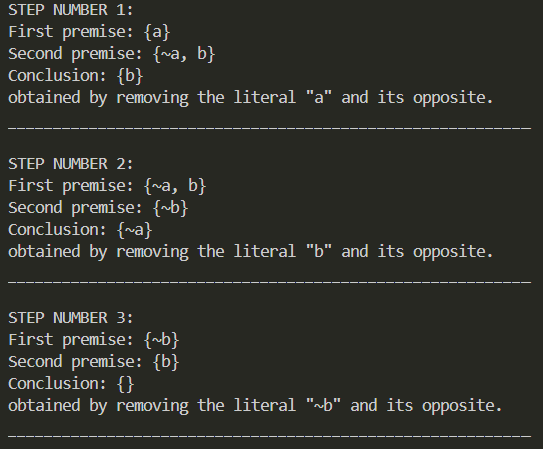
\includegraphics[width=0.7\textwidth, height=0.4\textheight]{img/step.png}
\end{figure} 
Come si può notare, nello step 3 viene trovata la clausola vuota, quindi in questo caso il metodo restituisce \texttt{false} (\texttt{s} è \textbf{insoddisfacibile}).


% 
% 
%			CAPITOLO 4
\chapter{Implementazione in Java di formule generiche}
\label{formulas}
Finora ci siamo concentrati soltanto su formule espresse in \emph{CNF} rappresentate mediante la classe \texttt{ClauseSet}. Se volessimo implementare una formula qualsiasi della logica proposizionale sono necessari altri elementi. I package \emph{formula} e \emph{connective} del progetto Java visto nella sezione \ref{project_structure} contengono i file necessari per rappresentare le formule della logica proposizionale. Se si volesse verificare la soddisfacibilità di una formula, è necessario convertire prima la formula in \emph{CNF} (ottenendo così l'istanza di \texttt{ClauseSet} associata), e poi richiamare il metodo \texttt{isSatisfiable} della classe \texttt{Resolution} dando in input quella istanza. Questo aspetto viene affrontato nella sezione \ref{clausification}.

\section{La classe astratta \texttt{Formula}}
Come visto nel capitolo \ref{intro}, una formula può essere \emph{atomica} o \emph{composta}, perciò nell'implementazione in Java è stata scritta la classe astratta \texttt{Formula}, che viene estesa dalle classi concrete \texttt{AtomicFormula} e \texttt{CompoundFormula}.

La classe \texttt{Formula} contiene soltanto il metodo astratto \texttt{toCnf} che permette di convertire la formula in \emph{CNF}, restituendo l'istanza di \texttt{ClauseSet} corrispondente (si veda la sezione \ref{clausification}).

\section{La classe \texttt{AtomicFormula}}
\label{AtomicFormula}
Questa classe estende \texttt{Formula} ed istanzia una formula atomica. Essa contiene un campo \texttt{atm} di tipo \texttt{Atom} che lo identifica, e alcuni semplici metodi per la sua gestione: il metodo per ottenere il nome (\texttt{getName}), il metodo per ottenere il letterale associato (\texttt{toLiteral}), e i classici metodi \texttt{equals} e \texttt{toString}.

\section{L'enumerazione \texttt{Connective}}
Prima di considerare la classe \texttt{CompoundFormula} è bene vedere prima l'enumerazione \texttt{Connective}. Essa si trova nel package \emph{connective} e definisce delle costanti enumerative che descrivono i connettivi della logica proposizionale usati dalle formule composte. La seguente tabella mostra le costanti associate alla loro rappresentazione testuale (ottenute dal metodo \texttt{toString}):
\begin{table}[H]
    \centering
    \begin{tabular}{|c||c|}
        \hline
        \textbf{Costante enumerativa} & \textbf{Rappresentazione testuale} \\
        \hline\hline
        NOT & $\sim$ \\
        \hline
        AND & $\&$ \\
        \hline
        OR & $|$ \\
        \hline
        IMPLIES & $-\!>$ \\
        \hline
        IFF & $<\!-\!>$ \\
        \hline
    \end{tabular}
\end{table}

\section{La classe \texttt{CompoundFormula}}
Questa classe estende \texttt{Formula} ed istanzia una formula composta, utilizzando le costanti dell'enumerazione \texttt{Connective}. Per la rappresentazione interna di una formula composta si usa un albero binario, che definisce la sua struttura ricorsiva. La radice dell'albero contiene il connettivo principale della formula, i nodi interni contengono i connettivi delle sue sottoformule, ed infine le foglie contengono le sue formule atomiche. I nodi che contengono i connettivi binari hanno due figli, mentre i nodi che contengono i connettivi unari hanno un solo figlio (il figlio sinistro).

Consideriamo il seguente esempio di formula:
\[\lnot(a \land b) \to (c \lor \lnot d)\]
La sua rappresentazione ad albero è la seguente:
\begin{figure}[H]
    \centering
    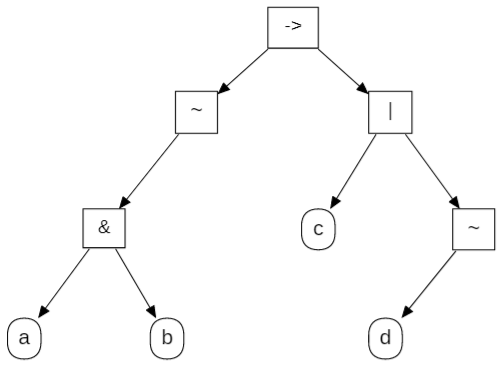
\includegraphics[width=0.7\textwidth, height=0.4\textheight]{img/albero.png}
\end{figure}
In questo albero, la radice è il nodo ``$-\!>$'', perché è il connettivo principale della formula dell'esempio. I nodi ``$\thicksim$'' hanno solo il figlio sinistro perché rappresentano la negazione, e le foglie sono le atomiche \emph{a, b, c, d}.

La classe \texttt{CompoundFormula} ha quindi come attributi il campo \texttt{mainConnective} che definisce il connettivo principale, e il campo \texttt{subFormulas} che consiste in un array di formule che contiene i nodi figli. La classe contiene dei metodi getter per ottenere il connettivo, il figlio destro ed il figlio sinistro, e sovrascrive i metodi \texttt{toString} e \texttt{toCnf}.

\section{Clausificazione di una formula}
\label{clausification}
Come spiegato all'inizio di questo capitolo, se volessimo verificare la soddisfacibilità di una formula \emph{F} tramite il metodo di risoluzione, è fondamentale effettuare prima la \emph{clausificazione} di \emph{F}, ovvero la sua conversione in \emph{CNF}, in modo tale da ottenere l'insieme di clausole necessario per il metodo di risoluzione. Per fare ciò bisogna applicare alcune regole di inferenza:
\begin{itemize}
    \item \textbf{Eliminazione della doppia implicazione}: 
    \[
    (p \tto q) \quad \equiv \quad ((p \to q) \land (q \to p))
    \]
    
    \item \textbf{Eliminazione dell'implicazione}: 
    \[
    (p \to q) \quad \equiv \quad (\lnot p \lor q)
    \]
    
    \item \textbf{Proprietà distributiva di or su and}:
    \[
    (p \lor (q \land r)) \quad \equiv \quad ((p \lor q) \land (p \lor r))
    \]
    
    \item \textbf{Doppia negazione}:
    \[
    \lnot\lnot p \quad \equiv \quad p
    \]
    
    \item \textbf{Leggi di De Morgan}:
    \[
    \lnot(p \land q) \quad \equiv \quad (\lnot p \lor \lnot q)
    \]
    \[
    \lnot(p \lor q) \quad \equiv \quad (\lnot p \land \lnot q)
    \]
\end{itemize}
Le regole appena mostrate vengono applicate in una delle implementazioni del metodo astratto \texttt{toCnf} della classe \texttt{Formula}. Questo metodo restituisce un \texttt{ClauseSet} e ha due diverse implementazioni: una per le formule atomiche e una per le formule composte.

L'implementazione del metodo \texttt{toCnf} nella classe \texttt{AtomicFormula} è molto semplice: esso restituisce un \texttt{ClauseSet} contenente una sola clausola, tale clausola contiene soltanto il letterale associato a quella formula atomica.
 
L'implementazione del metodo nella classe \texttt{CompoundFormula} invece applica sulla formula le regole di inferenza sopra citate, seguendo un approccio ricorsivo. Per la creazione del \texttt{ClauseSet} da restituire, utilizza i metodi \texttt{union} delle classi \texttt{Clause} e \texttt{ClauseSet}.

\subsection{Esempio di clausificazione}
Consideriamo la seguente formula:
\[ (a \lor b) \to c \]
la clausificazione viene fatta in tre passaggi:

\begin{itemize}
    \item Eliminazione implicazione:
    \[ \lnot (a \lor b) \lor c \]
    \item De Morgan:
    \[ (\lnot a \land \lnot b) \lor c \]
    \item Proprietà distributiva:
    \[ (\lnot a \lor c) \land (\lnot b \lor c) \]
\end{itemize}
La formula ricavata nell'ultimo passaggio è in \emph{CNF}, ed essa corrisponde all'insieme di clausole:
\[ \{ \quad \{\lnot a, c\}, \{\lnot b, c\} \quad \} \]

\section{Parsing di formule}
\label{parsing}
Se volessimo utilizzare un programma che legge da un flusso di input una formula in formato testuale (ad esempio da \emph{Stdin} o da un file di testo), è necessario interpretare la stringa di testo in modo tale da ottenere la formula. La trasformazione di rappresentazioni testuali in strutture dati utilizzabili da un programma è un processo noto come \emph{parsing}. Nel nostro sistema, implementiamo un parser per convertire le formule da stringhe di testo in oggetti di tipo \texttt{Formula}. Per eseguire il parsing, bisogna definire prima di tutto una grammatica che descrive il linguaggio utilizzato per le formule. A partire dalla grammatica vengono generati il \emph{lexer}, il \emph{parser} e il \emph{listener}.


\subsection{Utilizzo del parser ANTLR4}
Il parser utilizzato nel nostro sistema è \emph{ANTLR4}. Nella struttura del progetto presente nella sezione \ref{project_structure}, nel package \emph{antlr4} è presente il file \emph{FormulaExpression.g4} che contiene la grammatica. Inoltre, sono presenti quattro file che sono stati generati automaticamente da \emph{ANTLR4} a partire dalla grammatica:
\begin{itemize}
    \item \textbf{FormulaExpressionLexer.java}:
    esso consiste nel lexer, ovvero l'analizzatore lessicale; il suo scopo è quello di analizzare la stringa in input ed ottenere da esso un flusso di \emph{token}. In questo caso i token sono i connettivi, le variabili atomiche, e i caratteri di \emph{white space}.
    \item \textbf{FormulaExpressionParser.java}:
    esso consiste nel parser, che esegue l'analisi sintattica della stringa in input generando un \textbf{albero sintattico} (\emph{AST}), fondamentale per la costruzione della formula.
    \item \textbf{FormulaExpressionListener.java}:
    è un'interfaccia che definisce i metodi che vengono richiamati durante l'attraversamento dell'\emph{AST}.
    \item \textbf{FormulaExpressionBaseListener.java}:
    è una classe che implementa l'interfaccia \texttt{FormulaExpressionListener}, dove ogni metodo sovrascritto non esegue alcuna operazione.
\end{itemize}

Oltre a questi file, ne sono presenti altri due:
\begin{itemize}
    \item \textbf{FormulaListenerImplementation.java}:
    è una classe che estende il Base Listener. Utilizza uno \emph{stack} di formule come campo per la creazione delle sottoformule, e sovrascrive alcuni metodi del Base Listener.
    \item \textbf{ParseFormula.java}:
    è una classe che contiene soltanto il metodo \texttt{parse}. Esso è il metodo principale che prende in input una stringa, e mette insieme tutte le componenti viste precedentemente, creando tutto l'occorrente per il parsing. Infine restituisce la formula ottenuta a partire dalla stringa in input.
\end{itemize}

\subsubsection{La grammatica utilizzata}

Nel codice \ref{grammar} è presente il contenuto del file \emph{FormulaExpression.g4} che descrive la grammatica.

\begin{minipage}{\linewidth}
    \small
    \begin{lstlisting}[label=grammar, caption={file FormulaExpression.g4}]
grammar FormulaExpression;

start : formula EOF;

formula : atomic_formula
        | '(' formula ')' 
        | unary_connective formula
        | formula binary_connective formula
        ;

atomic_formula : LITERAL ;

unary_connective : NOT ;

binary_connective : AND | OR | IMPLIES | IFF;

//token
AND : '&' ;
OR : '|' ;
IMPLIES : '->' ;
NOT : '~' ;
IFF : '<->';

LITERAL : [a-z]+ ;
WS : [ \t\r\n]+ -> skip ;
    \end{lstlisting}
\end{minipage}
In questa grammatica ci sono le regole che definiscono le formule atomiche e composte, e le regole che descrivono i connettivi unari e binari. Le sottoformule sono distinguibili grazie alle parentesi tonde, che specificano anche la precedenza tra i vari connettivi della formula. in fondo al file è presente la definizione dei token. È bene notare che la rappresentazione testuale dei connettivi in questa grammatica è la medesima utilizzata dall'enumerazione \texttt{Connective}.

\subsubsection{Esempio di \emph{AST}}
Consideriamo la seguente formula rappresentata mediante una stringa:
\[ (a \; \& \; \sim\!b) \quad -\!> \quad c \]
se eseguiamo il parsing di questa stringa otteniamo il seguente \emph{AST}:
\begin{figure}[H]
    % \centering
    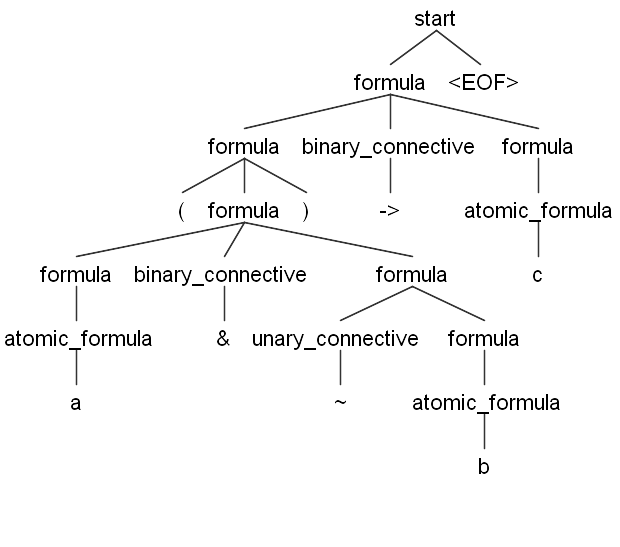
\includegraphics[width=0.7\textwidth, height=0.5\textheight]{img/antlr4_parse_tree.png}
\end{figure}
Durante l'attraversamento di questo albero vengono eseguiti i metodi \\ \texttt{ExitAtomic\_formula} e \texttt{exitFormula} della classe \texttt{FormulaListenerImplementation}; essi vengono richiamati rispettivamente quando si esce da un nodo \emph{atomic\_formula} e da un nodo \emph{formula}. Nel primo caso si crea una formula atomica e la si aggiunge allo \emph{stack} (tramite l'operazione di \emph{push}), nel secondo caso si controlla la presenza di un figlio che contiene un connettivo unario o binario, e si crea una formula composta applicando quel connettivo alla formula in cima allo stack (nel caso di connettivo unario) oppure alle prime due formule in cima allo stack (nel caso di connettivo binario). Infine viene inserita nello stack la formula appena creata. Per ottenere l'elemento in cima allo stack viene usata l'operazione di \emph{pop} su di esso.

Alla fine della visita dell'\emph{AST}, in cima allo stack ci sarà la formula associata alla stringa di partenza, che viene ottenuta dal metodo \texttt{getFormula} e a sua volta restituita dal metodo \texttt{parse} (si veda il codice \ref{parse}). Nell'esempio visto in precedenza la formula ottenuta è:
\[ (a \land \lnot b) \to c \]

\begin{minipage}{\linewidth}
    \begin{lstlisting}[caption={Metodo \texttt{parse} della classe \texttt{ParseFormula}}, label={parse}]
public static Formula parse(String formulaStr) {
    CharStream input = CharStreams.fromString(formulaStr);
    FormulaExpressionLexer lexer = new FormulaExpressionLexer(input);
    CommonTokenStream tokens = new CommonTokenStream(lexer);
    FormulaExpressionParser parser = new FormulaExpressionParser(tokens);

    //create listener
    FormulaListenerImplementation listener = new FormulaListenerImplementation();

    //adds the listener to the parser
    parser.addParseListener(listener);

    try {
        //analyze the input and get the corresponding formula
        parser.start();
        return listener.getFormula();
    } catch (Exception e) {
        return null;
    }
}
    \end{lstlisting}
\end{minipage}


% 
% 
%			CAPITOLO 5
\chapter{Logiche modali non-normali ed estensione del metodo di risoluzione}
\label{modal}
Questo capitolo si concentra sulle logiche modali, in particolare su quelle non-normali, e su come estendere il metodo di risoluzione per questo tipo di logiche. La prima parte del capitolo illustra le nozioni teoriche, la seconda parte riguarda l'implementazione in Java di quello che viene spiegato nella parte teorica. 

\begin{definition}
    Una logica modale è un'estensione della logica classica che introduce connettivi modali per esprimere modalità come necessità e possibilità. Questi connettivi permettono di ragionare non solo sulle proposizioni, ma anche su ciò che è possibile o necessario in vari mondi possibili.
\end{definition}
Il connettivo modale che noi consideriamo è il \emph{box} ($\Box$); esso viene utilizzato nelle formule delle logiche modali, insieme agli altri connettivi della logica classica. Questo connettivo è fondamentale nella formalizzazione di concetti come la necessità, l'obbligatorietà, la conoscenza o la verità assoluta, a seconda del contesto in cui viene utilizzato.

\section{Panoramica sulle logiche modali non-normali}
Le logiche modali \emph{non-normali} (\emph{NNML}) sono una classe di sistemi logici che estendono la logica modale normale introducendo concetti e assiomi che non sono presenti nella forma più basilare della logica modale. Queste logiche \emph{non-normali} si discostano dalle proprietà della logica modale \emph{normale} minima, \textbf{K}, che soddisfa tutti gli assiomi basilari della logica modale. Queste logiche sono organizzate gerarchicamente in un ``cubo'' di sistemi logici, che comprende la logica modale \textbf{E} come la più semplice e altre logiche ottenute aggiungendo assiomi come \textbf{C}, \textbf{M} e \textbf{N}. Il metodo di risoluzione che vediamo in questo capitolo si concentra soltanto sulla logica modale non-normale minimale \textbf{E}.

Gli assiomi della logica minimale \textbf{E} comprendono gli assiomi della logica classica e la regola di congruenza \textbf{RE}: da $\phi \tto \psi$ si inferisce $\Box \phi \tto \Box \psi$, dove $\phi$ e $\psi$ sono due formule.

\section{Forma clausale}
La forma clausale di una formula $\phi$ consiste nell'esprimere $\phi$ come un insieme di clausole, come nel caso della logica classica.
\subsection*{Letterali}
I letterali possono essere di due tipi: \emph{proposizionali} o \emph{modali}. I letterali proposizionali sono i medesimi della logica classica (si veda sezione \ref{CNF}); i letterali modali sono della forma $\Box p$ oppure $\lnot \Box p$, dove $p$ è una variabile proposizionale.
\subsection*{Clausole}
Le clausole, come nella logica classica, sono una disgiunzione di letterali. Questa volta però le clausole possono essere di due tipi: 
\begin{itemize}
    \item \textbf{Clausola locale}: \[ l_1 \lor l_2 \lor \ldots \lor l_n \]
    \item \textbf{Clausola globale}: \[ G(l_1 \lor l_2 \lor \ldots \lor l_n) \]
\end{itemize}
dove $l_i$ è un letterale proposizionale o modale. Una clausola globale è vera in tutti i mondi di un modello, una clausola locale invece è vera soltanto in un mondo del modello. Anche in questo caso è possibile utilizzare la notazione insiemistica per rappresentare le clausole.

\section{Clausificazione di formule modali}
\label{modal_claus}
Per poter effettuare la clausificazione di una formula $\phi$ è necessario utilizzare la funzione $\eta$. Essa è una funzione iniettiva di rinominazione, il cui scopo è quello di mappare una nuova variabile proposizionale ad ogni sottoformula di $\phi$; è importante che questa nuova variabile non sia presente in $\phi$. La funzione $\eta$ viene utilizzata all'interno di un'altra funzione, chiamata \textbf{R}, ossia la funzione di \emph{riduzione}. La clausificazione della formula $\phi$ viene fatta nel seguente modo:
\[ \{ \eta(\phi) \} \cup R(G(\eta(\phi) \tto \phi)) \]
dove \textbf{R} è così definita (si consideri $t$ e $p$ come variabili proposizionali):
\[
\begin{aligned}
R(G(t \tto p)) &= \{ G(\lnot t \lor p), G(t \lor \lnot p) \} \\
R(G(t \tto \lnot \psi)) &= \{ G(\lnot t \lor \lnot \eta(\psi)), G(t \lor \eta(\psi)) \} \cup R(G(\eta(\psi) \tto \psi)) \\
R(G(t \tto \psi \lor \psi')) &= \{ G(\lnot t \lor \eta(\psi) \lor \eta(\psi')), G(t \lor \lnot \eta(\psi)), G(t \lor \lnot \eta(\psi')) \} \\
& \quad \cup R(G(\eta(\psi) \tto \psi)) \cup R(G(\eta(\psi') \tto \psi')) \\
R(G(t \tto \Box \psi)) &= \{ G(\lnot t \lor \Box \eta(\psi)), G(t \lor \lnot \Box \eta(\psi)) \} \cup R(G(\eta(\psi) \tto \psi))
\end{aligned}
\]
Essa è una funzione ricorsiva, in cui il caso base è rappresentato da $R(G(t \tto p))$. La clausola $\{\eta(\phi)\}$ è una clausola locale che contiene soltanto la variabile proposizionale associata alla formula $\phi$, ossia $\eta(\phi)$. L'insieme di clausole che contiene solo questa clausola viene unito ad un altro insieme di clausole ottenuto ricorsivamente dalla funzione \textbf{R} applicata alla formula globale $G(\eta(\phi) \tto \phi)$. Si noti che questa funzione è definita solamente per formule $\phi$ che contengono i connettivi \emph{not}, \emph{or} e \emph{box}. Gli altri connettivi binari possono essere ricavati utilizzando i connettivi \emph{or} e \emph{not}.

\subsection*{Esempio di clausificazione}
Consideriamo la seguente formula $\phi$:
\[
    \phi = \Box(\lnot a \lor b)
\]
Prima di procedere con la clausificazione dobbiamo vedere quali sono le nuove variabili proposizionali ottenute dalla funzione di rinominazione $\eta$ su ogni sottoformula $\psi$. La tabella \ref{tab:eta} mostra questa mappatura. Si noti che $\phi$ è una sottoformula di se stessa.

\begin{table}[H]
    \centering
    \begin{tabular}{|c|c|}
        \hline
        $\psi$ & $\eta(\psi)$ \\
        \hline\hline
        $\Box(\lnot a \lor b)$ & $\$p_0$ \\
        \hline
        $\lnot a \lor b$ & $\$p_1$ \\
        \hline
        $\lnot a$ & $\$p_2$ \\
        \hline
        $a$ & $\$p_3$ \\
        \hline
        $b$ & $\$p_4$ \\
        \hline
    \end{tabular}
    \caption{Funzione $\eta$ applicata su tutte le sottoformule $\psi$ di $\phi$}
    \label{tab:eta}
\end{table}
Di seguito viene mostrato l'elenco degli step per effettuare la clausificazione.
\begin{enumerate}
    \item Si ottiene la clausola locale $\{\eta(\phi)\}$: \[ \{\$p_0\} \]
    \item A questa clausola si aggiungono le clausole globali ottenute da $R(G(\eta(\phi) \tto \phi))$:
    \[G(\{\lnot \$p_0, \Box \$p_1\})\]
    \[G(\{\$p_0, \lnot \Box \$p_1\})\]
    \item Si aggiungono le clausole ottenute da $R(G(\eta(\psi) \tto \psi))$, dove $\psi = \lnot a \lor b$:
    \[G(\{\lnot \$p_1, \$p_2, \$p_4\})\]
    \[G(\{\$p_1, \lnot \$p_2\})\]
    \[G(\{\$p_1, \lnot \$p_4\})\]
    \item Si aggiungono le clausole ottenute da $R(G(\eta(\psi) \tto \psi))$ e da $R(G(\eta(\psi') \tto \psi'))$ dove $\psi = \lnot a$ e $\psi' = b$. Consideriamo $R(G(\eta(\psi) \tto \psi))$, si ottengono le seguenti clausole:
    \[G(\{\lnot \$p_2, \lnot \$p_3\})\]
    \[G(\{\$p_2, \$p_3\})\]
    \item Si aggiungono le clausole ottenute da $R(G(\eta(\psi) \tto \psi))$, dove $\psi = a$ (\textbf{caso base}):
    \[G(\{\lnot \$p_3, a\})\]
    \[G(\{\$p_3, \lnot a\})\]
    \item Ritorniamo allo step 4, e consideriamo $R(G(\eta(\psi') \tto \psi'))$ (\textbf{caso base}). Si aggiungono le seguenti clausole:
    \[G(\{\lnot \$p_4, b\})\]
    \[G(\{\$p_4, \lnot b\})\]
\end{enumerate}
Nella sezione \ref{clausification_impl}, che riguarda l'implementazione della clausificazione, vedremo che è possibile semplificare la clausificazione di una formula in modo da ottenere meno clausole rispetto a quelle che si otterrebbero applicando la clausificazione come sopra riportato.

\section{Metodo di Risoluzione per logiche modali non-normali}
Il metodo di risoluzione per le logiche modali non-normali è un approccio sistematico per determinare la soddisfacibilità delle formule (espresse in forma clausale) di queste logiche. Esso rappresenta un'estensione del metodo di risoluzione per la logica classica, che considera l'utilizzo di clausole locali e globali, e l'applicazione di regole di risoluzione adattate ad una logica $L$ presa in esame ($RES_L$). Come nella logica classica, si considerano tutte le coppie di clausole e si cerca di trovare la contraddizione applicando le regole. Qui ci concentriamo solo sulle regole per la logica modale minimale \textbf{E}, ovvero $RES_E$.

\subsection{Regole di risoluzione per la logica modale \emph{E}}
Nelle regole $RES_E$ che vediamo ora, $C$ e $D$ sono clausole, $l$ è un letterale, e $p$ è una variabile proposizionale. Le regole $RES_E$ sono le seguenti:

% \[
%     \AXC{$(D \lor l)$}
%     \AXC{$(D' \lor \lnot l)$}
%     \RightLabel{LRES}
%     \BIC{$(D \lor D')$}
%     \DP
% \]

% \[
%     \AXC{$G(D \lor l)$}
%     \AXC{$G(D' \lor \lnot l)$}
%     \RightLabel{GRES}
%     \BIC{$G(D \lor D')$}
%     \DP
% \]

% \[
%     \AXC{$G(D)$}
%     \RightLabel{G2L}
%     \UnaryInfC{$D$}
%     \DP
% \]

% \begin{prooftree}
%     \AXC{$(D \lor \Box p)$}
%     \AXC{$(D' \lor \lnot \Box p')$}
%     \AXC{$G(C)$}
%     \AXC{$G(C')$}
%     \RightLabel{LERES}
%     \QuaternaryInfC{$(D \lor D')$}
% \end{prooftree}
    
% \begin{prooftree}
%     \AXC{$G(D \lor \Box p)$}
%     \AXC{$G(D' \lor \lnot \Box p')$}
%     \AXC{$G(C)$}
%     \AXC{$G(C')$}
%     \RightLabel{GERES}
%     \QuaternaryInfC{$G(D \lor D')$}
% \end{prooftree}    

\begin{align*}
    \textbf{LRES} & \quad \frac{(D \lor l) \quad (D' \lor \lnot l)}{(D \lor D')} \\[10pt]
    \textbf{GRES} & \quad \frac{G(D \lor l) \quad G(D' \lor \lnot l)}{G(D \lor D')} \\[10pt]
    \textbf{G2L} & \quad \frac{G(D)}{D} \\[10pt]
    \textbf{LERES} & \quad \frac{(D \lor \Box p) \quad (D' \lor \lnot \Box p') \quad G(C) \quad G(C')}{(D \lor D')} \\[10pt]
    \textbf{GERES} & \quad \frac{G(D \lor \Box p) \quad G(D' \lor \lnot \Box p') \quad G(C) \quad G(C')}{G(D \lor D')} \\[10pt]
    & \text{dove } C \subseteq (\lnot p \lor p') \text{ e } C' \subseteq (p \lor \lnot p')
\end{align*}

Di seguito viene riportata la descrizione di ogni regola:
\begin{itemize}
    \item \textbf{LRES}: Questa regola è la medesima della regola \emph{Res} della logica classica (si veda sezione \ref{Res}), con la differenza che le due premesse e la risolvente sono clausole locali, e che $l$ presente nelle premesse può essere un letterale modale.
    \item \textbf{GRES}: Come \emph{LRES}, ma le due premesse e la risolvente sono clausole globali.
    \item \textbf{G2L}: Questa regola permette di ricavare una clausola locale a partire dalla sua controparte globale (la soddisfacibilità locale è conseguenza di quella globale).
    \item \textbf{LERES}: Questa regola afferma che i letterali modali $\Box p$ e $\lnot \Box p'$ possono essere considerati come l'uno l'opposto dell'altro ogni volta che i letterali proposizionali $p$ e $p'$ sono globalmente equivalenti. Questo avviene in tre casi: \begin{enumerate}
        \item quando $G(C) = G(\lnot p \lor p')$ e $G(C') = G(p \lor \lnot p')$, questo significa che $p$ e $p'$ sono semanticamente equivalenti (ossia $p \tto p'$).
        \item quando $G(C) = G(\lnot p)$ e $G(C') = G(\lnot p')$, in questo caso $p$ e $p'$ sono entrambi globalmente falsi, e quindi semanticamente equivalenti.
        \item quando $G(C) = G(p')$ e $G(C') = G(p)$, in questo caso $p$ e $p'$ sono entrambi globalmente veri, e quindi semanticamente equivalenti.
    \end{enumerate}
    Ogni volta che si rientra in uno di questi casi, si considera l'approccio classico della regola di risoluzione, ovvero si genera la risolvente cancellando i letterali modali $\Box p$ e $\lnot \Box p'$ dalle prime due premesse, e facendo l'unione. In questo caso le prime due premesse e la risolvente sono clausole locali (mentre le ultime due premesse devono essere sempre globali).
    \item \textbf{GERES}: Come \emph{LERES}, ma le prime due premesse e la risolvente sono clausole globali.
\end{itemize}

\section*{Implementazione in Java}
Ora vediamo la seconda parte di questo capitolo, che si concentra sull'implementare in Java i concetti che abbiamo visto finora nel capitolo. La struttura del progetto Java è simile a quella del progetto per la logica classica (si veda sezione \ref{project_structure}), e anche alcune classi sono simili a quelle della logica classica.

\section{Implementazione della forma clausale}
\subsection*{Le classi per i letterali}
Come nell'implementazione per la logica classica, è presente la classe astratta \texttt{Literal} (si veda sezione \ref{literal}). Questa classe viene estesa dalle classi \texttt{PropAtom} e \texttt{NegPropAtom} che rappresentano i letterali proposizionali, e dalle classi \texttt{ModalAtom} e \texttt{NegModalAtom} che rappresentano i letterali modali. Per la rappresentazione testuale dei letterali modali si usa il carattere ``$\#$'', ad esempio ``$\#p$'' o ``$\sim\!\#q$''.

\subsection*{Le classi per le clausole}
Per quanto riguarda le clausole, è presente la classe astratta \texttt{Clause}. Questa classe è simile a quella utilizzata nella logica classica (si veda sezione \ref{Clause}), con la differenza che in questo caso si tratta di una classe astratta che definisce il metodo astratto \texttt{union}; gli altri metodi sono gli stessi della classe \texttt{Clause} per la logica classica.

La classe \texttt{Clause} viene estesa dalle due classi \texttt{LocalClause} e \texttt{GlobalClause}, che rappresentano rispettivamente le clausole locali e globali. Queste due classi forniscono un'implementazione del metodo \texttt{union}, infatti una clausola di un tipo (locale o globale) può essere unita soltanto con un'altra clausola dello stesso tipo. Inoltre le due classi sovrascrivono i metodi \texttt{equals} e \texttt{toString} (nella rappresentazione testuale delle clausole globali viene usato ``G($\cdot$)'').

\subsection*{La classe \texttt{ClauseSet}}
La classe \texttt{ClauseSet} rappresenta la forma clausale di una formula, espressa come insieme di clausole. Questa classe è la medesima utilizzata nella logica classica (si veda sezione \ref{ClauseSet}). La differenza sostanziale è che le clausole all'interno di un'istanza di \texttt{ClauseSet} possono essere indistintamente locali o globali, e i letterali contenuti in ciascuna clausola possono essere parimenti proposizionali o modali.


\section{implementazione delle formule modali}
Per l'implementazione delle formule modali generiche si segue lo stesso approccio usato per la logica classica (si veda l'inizio del capitolo \ref{formulas}); quindi si usa la classe astratta \texttt{Formula} che viene estesa dalle classi \texttt{AtomicFormula} e \texttt{CompoundFormula}. La classe \texttt{AtomicFormula} è identica a quella presentata nella sezione \ref{AtomicFormula}. La classe \texttt{CompoundFormula} utilizza l'enumerazione \texttt{Connective} estesa al connettivo unario \emph{box} (si utilizza la costante enumerativa \texttt{BOX}, la cui rappresentazione testuale usa il carattere ``$\#$''). La classe \texttt{AtomicFormula} implementa le formule seguendo lo stesso approccio con alberi binari che abbiamo già visto; i nodi che descrivono il connettivo \emph{box} hanno solo il figlio sinistro, come nel caso del \emph{not} (perché è unario).

\subsection{Implementazione della clausificazione}
\label{clausification_impl}
\subsubsection{La classe \texttt{Eta}}
La clausificazione viene fatta utilizzando la classe \texttt{Eta}, essa gestisce l'esecuzione della funzione di rinominazione $\eta$. Questa classe ha come campo una mappa che associa istanze di \texttt{Formula} a istanze di \texttt{PropAtom}; il costruttore della classe prende in input un oggetto \texttt{Formula} $f$ e crea ricorsivamente la mappa associando ad ogni sottoformula di $f$ una nuova variabile proposizionale (\texttt{PropAtom}), i nomi che vengono dati alle variabili atomiche sono $\$p1, \$p2, \dots, \$pi$.

La classe \emph{Eta} ha il metodo \texttt{getPropVariable} che prende in input un oggetto \texttt{Formula} $f$ e restituisce il valore $\eta(f)$. Un'istanza di \texttt{Eta} viene usata come campo statico all'interno della classe \texttt{Formula}.

\subsubsection{I metodi per la clausificazione}
La classe \texttt{CompoundFormula} permette di eseguire la clausificazione tramite i metodi \texttt{toClauseSet}, \texttt{R} e \texttt{classicClausification}. La clausificazione viene implementata in maniera leggermente diversa rispetto a quanto riportato in questo capitolo (nella sezione \ref{modal_claus}), infatti è possibile considerare $\eta(p) = p$ nel caso in cui $p$ sia una formula atomica (\texttt{AtomicFormula}); in questo modo si evita il caso $R(G(\eta(p) \tto p))$. Inoltre, è possibile applicare la clausificazione della logica classica quando la funzione \textbf{R} arriva a calcolare $R(G(\eta(F) \tto F))$, dove $F$ è una formula della logica classica (ossia non contiene il connettivo \emph{box}); in questo caso si fa la clausificazione classica della formula $\eta(F) \tto F$, che consiste in un caso base della funzione \textbf{R}. Si può applicare la clausificazione classica anche quando la formula $F$ contiene il connettivo \emph{box} ma solo se esso viene applicato alle atomiche della formula. Ad esempio, se avessimo la formula $(\Box a \land b) \to \Box c$, possiamo applicare su di essa la clausificazione classica, senza usare la funzione $\eta$.

Vediamo ora una descrizione dei metodi usati per la clausificazione.

\subsubsection{Il metodo \texttt{toClauseSet}}
Questo metodo è il primo ad essere richiamato per la clausificazione, ed è l'unico dei tre ad essere pubblico. Esso controlla se la formula \texttt{this} da clausificare è classica, in tal caso richiama il metodo \texttt{classicClausification}. Se invece non è classica, procede con la parte iniziale della clausificazione con $\eta$: crea una nuova istanza del campo statico \texttt{Eta} (della \emph{superclasse} \texttt{Formula}), e crea un nuovo \texttt{ClauseSet} vuoto nel quale aggiunge la clausola locale $\{\eta(this)\}$, ed infine restituisce l'unione con il \texttt{ClauseSet} ottenuto da $R(G(\eta(this) \tto this))$. Il codice \ref{toClauseSet} mostra questo metodo.

\subsubsection{Il metodo \texttt{R}}
Il metodo \texttt{R} prende in input l'oggetto \texttt{PropAtom t} corrispondente alla rinominazione della formula sulla quale viene richiamato il metodo, ad esempio: scrivere \texttt{this.R(t)} equivale ad applicare $R(G(t \tto this))$, dove $t = \eta(this)$. Il metodo applica la funzione \textbf{R} in maniera ricorsiva come abbiamo visto, tenendo conto anche dei casi di doppia negazione (questo capita quando si calcola $R(G(t \tto \lnot \lnot \psi))$), ed evita di calcolare $R(G(p \tto p))$ (dove $p$ è atomica) fermandosi alla chiamata ricorsiva precedente. Inoltre considera come caso base il calcolo di $R(G(t \tto F))$ dove $F$ è una formula della logica classica (richiamando in questo caso il metodo \texttt{classicClausification} su $t \tto F$). Siccome questo metodo è lungo, il codice \ref{R} riporta soltanto il caso in cui viene calcolato $R(G(t \tto \lnot \psi))$; in questo codice la variabile \texttt{psi} è il figlio sinistro della formula \texttt{this} (si noti che \texttt{this} è $\lnot \psi$), la variabile \texttt{etaPsi} è il valore $\eta(\texttt{psi})$ ed infine la variabile \texttt{res} è un \texttt{ClauseSet} inizialmente vuoto.

\subsubsection{Il metodo \texttt{classicClausification}}
\label{classicClausification}
Questo metodo esegue la clausificazione classica, applicando le regole di inferenza riportate nella sezione \ref{clausification}. Quindi il metodo \texttt{classicClausification} è uguale al metodo \texttt{toCnf} per la logica classica, con la differenza che tutte le clausole restituite sono globali; inoltre, gestisce anche le formule che contengono il connettivo \emph{box} solo se compare davanti alle atomiche (ad esempio se contengono $\Box p$ e/o $\lnot \Box q$).

Ad esempio, se dobbiamo clausificare la formula $\lnot(\Box p \lor \lnot \Box q)$ viene eseguito il metodo \texttt{classicClausification}, che restituisce il seguente insieme di clausole:
\[
    \{ \; G(\lnot \Box p), \; G(\Box q) \; \}
\]
In questo modo si evita di utilizzare le funzioni $\eta$ e \emph{R}, rendendo più semplice la clausificazione.

\begin{minipage}{\linewidth}
    % \small
    \begin{lstlisting}[caption={Metodo \texttt{toClauseSet} della classe \texttt{CompoundFormula}}, label={toClauseSet}]
@Override
public ClauseSet toClauseSet() {
    if (this.isClassic()) {
        return this.classicClausification();
    } else {
        eta = new Eta(this); //eta e' il campo statico della classe Formula.
        PropAtom t = eta.getPropVariable(this);
        ClauseSet cs = new ClauseSet(new LocalClause(t));
        return cs.union(this.R(t));
    }
}
    \end{lstlisting}
\end{minipage}

\begin{minipage}{\linewidth}
    \small
    \begin{lstlisting}[caption={Parte del metodo \texttt{R} della classe \texttt{CompoundFormula}}, label={R}]
switch (this.mainConnective) {
    case NOT:
        GlobalClause gc1 = new GlobalClause();
        gc1.add(t.getOpposite());
        gc1.add(etaPsi.getOpposite());
        res.add(gc1);
        GlobalClause gc2 = new GlobalClause();
        gc2.add(t);
        gc2.add(etaPsi);
        res.add(gc2);
        if (psi instanceof CompoundFormula) {
            CompoundFormula cf_psi = (CompoundFormula) psi;
            if (cf_psi.isClassic()) {
                CompoundFormula f = new CompoundFormula(IFF, new AtomicFormula(etaPsi), psi);
                return res.union(f.classicClausification());
            }
            return res.union(cf_psi.R(etaPsi));
        }
        return res;
    case OR:
        ...
}
    \end{lstlisting}
\end{minipage}

\section*{Parsing di formule modali}
Il parsing di formule modali viene fatto nello stesso modo che abbiamo visto nella sezione \ref{parsing}, in questo caso però si deve considerare il connettivo \emph{box}. Per farlo, bisogna modificare la grammatica presente nel codice \ref{grammar}, aggiungendo nella definizione dei token la riga:
\begin{center}
    \textbf{BOX} : '$\#$';
\end{center}
e modificando la regola \emph{unary$\_$connective} nel seguente modo:
\begin{center}
    \textbf{unary\_connective} : NOT $|$  BOX;
\end{center}
In questo modo l'\emph{AST} terrà conto anche del connettivo \emph{box}.

\section{Implementazione del metodo di risoluzione}
\label{impl_res_modal}
L'implementazione del metodo di risoluzione viene svolta, come nel caso della logica classica, all'interno della classe \texttt{Resolution}; essa è una classe senza costruttori dove sono presenti dei campi statici e metodi statici. I campi statici sono quelli descritti nella sezione \ref{class:Resolution}, ossia \texttt{visited}, \texttt{enableSteps} e \texttt{trace}. i metodi della classe sono i seguenti:
\begin{itemize}
    \item \texttt{isSatisfiable}
    \item \texttt{getComplementaryLiteral}
    \item \texttt{getModalLiterals}
    \item \texttt{addCoupleInMap}
    \item \texttt{alreadyVisited}
    \item \texttt{setEnableSteps}
    \item \texttt{printTrace}
    \item \texttt{G2L}
    \item \texttt{LRES}
    \item \texttt{GRES}
    \item \texttt{LERES}
    \item \texttt{GERES}
\end{itemize}
\subsection*{Il metodo \texttt{isSatisfiable}}
Il metodo \texttt{isSatisfiable} è il metodo principale che implementa l'algoritmo di risoluzione ed è l'unico ad essere pubblico. Questo metodo prende in input un oggetto \texttt{ClauseSet s} e restituisce \texttt{true} se \texttt{s} è soddisfacibile, \texttt{false} altrimenti. Inizialmente, Dopo aver controllato che \texttt{s} non sia \texttt{null} e non sia vuoto, elimina tutte le eventuali clausole tautologiche e crea la lista di clausole \texttt{listCl} dove aggiunge tutte le clausole rimaste in \texttt{s}. Lo svolgimento del metodo \texttt{isSatisfiable} può essere diviso in tre parti:

\begin{enumerate}
    \item \textbf{Applicazione della regola G2L}: ad ogni clausola globale contenuta in \texttt{listCl} viene applicata la regola \emph{G2L} (tramite il metodo \texttt{G2L}), e le nuove clausole ottenute vengono aggiunte a \texttt{listCl}.
    
    \item \textbf{Applicazione delle regole LRES e GRES}: vengono eseguiti due cicli \emph{for} innestati sulla lista \texttt{listCl} in modo da applicare (dove possibile) la regola \emph{LRES} su tutte le coppie di clausole locali, e la regola \emph{GRES} su tutte le coppie di clausole globali (tramite i metodi \texttt{LRES} e \texttt{GRES}). Per verificare il tipo di clausola si utilizza l'operatore \texttt{instanceof}, per ottenere il letterale $l$ (oppure $\lnot l$), si usa il metodo \texttt{getComplementaryLiteral}, il cui funzionamento è il medesimo dell'omonimo metodo spiegato nella sezione \ref{getComplementaryLiteral}. Ogni volta che vengono eseguite le regole \emph{LRES} e \emph{GRES} viene fatto un controllo sulla risolvente: se è vuota, il metodo restituisce \texttt{false}, altrimenti la risolvente viene aggiunta a \texttt{listCl} (se e solo se non è tautologica oppure non è già presente nella lista) e il metodo continua la sua esecuzione.
    
    \item \textbf{Applicazione delle regole LERES e GERES}: viene eseguito un altro paio di \emph{for} innestati sulla lista \texttt{listCl}, questa volta cercando di applicare (dove possibile) la regola \emph{LERES} su tutte le coppie di clausole locali, e la regola \emph{GERES} su tutte le coppie di clausole globali; infine esegue sulla risolvente le stesse operazioni del caso precedente ogni volta che viene applicata una delle due regole. Per poter ottenere i letterali modali $\Box p$ e $\lnot \Box p'$ necessari per attuare le regole \emph{LERES} e \emph{GERES}, si utilizza il metodo \texttt{getModalLiterals}. Il codice \ref{method:isSatisfiable} mostra la parte del metodo \texttt{isSatisfiable} dove sono presenti i due cicli \texttt{for} innestati per effettuare le regole \emph{LERES} e \emph{GERES}.
\end{enumerate}

\subsubsection{Il metodo \texttt{getModalLiterals}}
Questo metodo verifica se è possibile applicare le regole \emph{LERES} e \emph{GERES} all'interno del metodo \texttt{isSatisfiable}, ed in caso affermativo restituisce i due letterali modali $\Box p$ e $\lnot \Box p'$. Esso prende in input due clausole, una lista di clausole (nel nostro caso \texttt{listCl}) e restituisce un array di letterali (\texttt{Literal[]}). Il metodo controlla se in una delle due clausole in input sia presente un letterale modale positivo (\texttt{ModalAtom}), ed un letterale modale negativo (\texttt{NegModalAtom}); se ciò dovesse capitare, allora ispeziona la lista di clausole fornita in input (\texttt{listCl}) con lo scopo di ricercare le clausole $G(C)$ e $G(C')$, ovvero le ultime due premesse delle regole \emph{LERES} e \emph{GERES}. Se vengono trovate, allora il metodo \texttt{getModalLiterals} restituisce l'array contenente i due letterali modali, in caso contrario restituisce un array vuoto.

\subsection{Implementazione delle regole di risoluzione}
Le regole di risoluzione vengono implementate mediante gli omonimi metodi presenti nella classe \texttt{Resolution}.

\subsubsection{Il metodo \texttt{G2L}}
Il metodo \texttt{G2L} prende in input una clausola globale \texttt{gc}, e restituisce la corrispondente locale. Per farlo, istanzia una clausola locale vuota, e la riempie aggiungendo tutti i letterali presenti in \texttt{gc}.

\subsubsection{I metodi \texttt{LRES} e \texttt{GRES}}
Questi metodi sono implementati nello stesso modo del metodo \texttt{resolRule} della logica classica, con la differenza che nel caso di \texttt{LRES}, le due clausole in input (le clausole di premessa) e la clausola restituita (risolvente) sono locali, e nel caso di \texttt{GRES} le clausole in input e la clausola restituita sono globali. il codice \ref{method:LRES} mostra l'implementazione del metodo \texttt{LRES}.

\subsubsection{I metodi \texttt{LERES} e \texttt{GERES}}
Il metodo \texttt{LERES} prende in input due clausole locali e due letterali, e restituisce una clausola locale. Il metodo effettua l'unione delle due clausole, cancella i due letterali dal risultato, ed infine lo restituisce. Il metodo \texttt{GERES} effettua le stesse operazioni, ma le due clausole in input e la clausola restituita sono globali. il codice \ref{method:LERES} mostra l'implementazione del metodo \texttt{LERES}. Si noti che il metodo non controlla se i due letterali in input siano modali, questo perché ci si assicura che il metodo \texttt{isSatisfiable} richiami questo metodo con gli input corretti; inoltre, le due clausole $G(C)$ e $G(C')$ non vengono considerate, perché il metodo viene richiamato soltanto nel caso in cui \texttt{getModalLiterals} non restituisce un array vuoto.

\vspace{20pt}

\begin{minipage}{\linewidth}
    \small
    \begin{lstlisting}[caption={Metodo \texttt{LRES} della classe \texttt{Resolution}}, label={method:LRES}]
private static LocalClause LRES(LocalClause lc1, LocalClause lc2, Literal lit) {
    LocalClause result = (LocalClause) lc1.union(lc2);
    result.remove(lit);
    result.remove(lit.getOpposite());
    return result;
}
    \end{lstlisting}
\end{minipage}

\begin{minipage}{\linewidth}
    \small
    \begin{lstlisting}[caption={Metodo \texttt{LERES} della classe \texttt{Resolution}}, label={method:LERES}]
private static LocalClause LERES(LocalClause lc1, LocalClause lc2, Literal ma, Literal nma) {
    LocalClause result = (LocalClause) lc1.union(lc2);
    result.remove(ma);
    result.remove(nma);
    return result;
}
    \end{lstlisting}
\end{minipage}

\subsection{Memorizzazione delle coppie di clausole visitate}
La gestione delle coppie di clausole visitate viene fatta nello stesso modo in cui veniva svolto nell'implementazione per la logica classica (si veda la sezione \ref{visited}). Si utilizza quindi la mappa \texttt{visited}, che memorizza inizialmente le coppie di clausole sulle quali vengono applicate le regole \emph{LRES} e \emph{GRES} tramite i loro indici. Dopo che sono state applicate queste due regole su tutte le coppie possibili, la mappa \texttt{visited} viene svuotata, in questo modo sarà possibile eseguire le regole \emph{LERES} e \emph{GERES} anche sulle coppie di clausole alle quali sono state applicate in precedenza le altre due regole. Si noti che l'applicazione della regola \emph{G2L} non viene memorizzata.

Come nell'implementazione per la logica classica, viene utilizzato il metodo \\ \texttt{alreadyVisited} per verificare se una coppia di clausole è già stata visitata in precedenza; inoltre, per aggiungere una coppia alla mappa \texttt{visited} viene utilizzato il metodo \texttt{addCoupleInMap}

\subsection{Gestione degli step}
La gestione degli step viene svolta come nel caso della logica classica (si veda la sezione \ref{step}, nella quale vengono spiegati anche i metodi \texttt{setEnableSteps} e \texttt{printTrace}). In questo caso nella classe \texttt{Step} viene aggiunto, tra gli altri, un campo che specifica il nome della regola di risoluzione applicata nello step, e poi nel caso delle regole \emph{LERES} e \emph{GERES}, vengono aggiunte anche le premesse $G(C)$ e $G(C')$. La regola \emph{G2L} non viene presa in esame dagli step, perché è considerata sottintesa.

\begin{minipage}{\linewidth}
    \small
    \begin{lstlisting}[caption={cicli for innestati per l'esecuzione delle regole LERES e GERES nel metodo \texttt{isSatisfiable}}, label={method:isSatisfiable}]
for (int i = 0; i < listCl.size(); i++) {
    Clause c1 = listCl.get(i);
    int index1 = c1.getIndex();
    for (int j = 0; j < listCl.size(); j++) {
        Clause c2 = listCl.get(j);
        int index2 = c2.getIndex();
        if ((i != j) && (c1.getClass().equals(c2.getClass())) && !alreadyVisited(c1, c2)) {
            Literal[] literals = getModalLiterals(c1, c2, listCl);
            if (literals.length != 0) {
                addCoupleInMap(index1, index2);
                Clause resolvent = null;
                if ((c1 instanceof GlobalClause) && (c2 instanceof GlobalClause)) {
                    resolvent = GERES((GlobalClause) c1, (GlobalClause) c2, literals[0], literals[1]);
                    //gestione step
                } else {
                    resolvent = LERES((LocalClause) c1, (LocalClause) c2, literals[0], literals[1]);
                    //gestione step
                } 
                if (resolvent.isEmpty()) {
                    return false;
                }
                if (resolvent.isTautology()) {
                    //gestione step
                } else if (listCl.contains(resolvent)) {
                    //gestione step
                } else {
                    visited.put(resolvent.getIndex(), new HashSet<>());
                    listCl.add(resolvent);
                }
            }
        }
    }
}
    \end{lstlisting}
\end{minipage}

% 
% 
%			CAPITOLO 6
\chapter{Applicazioni pratiche del metodo di risoluzione}
\label{app}
Il metodo di risoluzione ha numerose applicazioni pratiche, tra cui:
\begin{itemize}
    \item \textbf{Verifica della validità di formule}: Determinare se una formula è valida all'interno di un dato sistema logico.
    \item \textbf{Dimostrazione automatica di teoremi}: Utilizzare algoritmi di risoluzione per automatizzare il processo di dimostrazione di teoremi.
    \item \textbf{Verifica formale}: Applicare metodi di risoluzione per verificare formalmente proprietà di sistemi hardware e software.
    \item \textbf{Soddisfacibilità booleana (SAT)}: Utilizzare il metodo di risoluzione per risolvere problemi di soddisfacibilità booleana, che hanno applicazioni in vari campi, tra cui l'intelligenza artificiale, la teoria dei giochi e la verifica del software.
\end{itemize}
L'utilizzo pratico che viene implementato nel nostro caso è quello della verifica della validità di formule logiche.

\begin{definition}
    Una formula F è \textbf{valida} se e solo se è una tautologia, ossia è vera in ogni interpretazione di F.
\end{definition}

\section{Verificare la validità di una formula}
Per verificare la validità di una qualsiasi formula $F$, si considera la sua negazione logica $\lnot F$ e si controlla se essa è soddisfacibile o meno; se $\lnot F$ è \textbf{insoddisfacibile}, allora $F$ è valida. Questo perché, come spiegato nel capitolo \ref{intro}, se applichiamo la negazione logica ad una tautologia otteniamo una contraddizione, e viceversa.

\subsection{Dimostrazione di conseguenze logiche}

\begin{definition}
    Siano $F_1$ e $F_2$ due formule. Si dice che $F_2$ è conseguenza logica di $F_1$ se e solo se per ogni interpretazione i, se i soddisfa $F_1$, allora soddisfa anche $F_2$. La conseguenza logica si può scrivere con $F_1 \models F_2$.
\end{definition}
Applicando la verifica della validità di formule, è possibile dimostrare la conseguenza logica di due formule $F_1$ e $F_2$ utilizzando l'implicazione logica, ovvero il connettivo $\to$. Infatti, se $F_2$ è conseguenza logica di $F_1$, allora la formula:
\[
    F_1 \to F_2
\]
è valida.
\subsubsection{Esempio di conseguenza logica}
Un esempio che possiamo considerare è il \emph{modus ponens}: siano $a, b$ due formule, se la formula $a \to b$ è vera, e anche $a$ è vera, allora la conseguenza $b$ è vera.

\[
    \AXC{$a$}
    \AXC{$a \to b$}
    \RightLabel{Modus ponens}
    \BIC{$b$}
    \DP
\]
Per dimostrare il modus ponens, creiamo una formula $F$ utilizzando la congiunzione logica per unire le due premesse ($a$ e $a \to b$), e l'implicazione logica per rappresentare la conseguenza logica (con $b$). La formula $F$ ottenuta è la seguente:
\[
    F \; = \; (a \land (a \to b)) \to b
\]
A questo punto dimostriamo la validità di $F$. Bisogna quindi verificare che la formula $\lnot F$ è insoddisfacibile. Per farlo, dobbiamo clausificare $\lnot F$ ed eseguire il metodo di risoluzione sull'insieme di clausole ottenuto. La clausificazione di $\lnot F$ produce il seguente insieme di clausole:
\[
    \{\quad \{a\}; \{\lnot a, b\}; \{\lnot b\} \quad\}
\]
applicando due volte la regola \emph{Res} si trova facilmente la clausola vuota. Questo dimostra che il modus ponens è valido nella logica classica.

\subsection{Dimostrazione di equivalenze logiche}
\begin{definition}
    Due formule $F_1$ e $F_2$ sono logicamente equivalenti se e solo se $F_1 \models F_2$ e $F_2 \models F_1$, ossia entrambe sono conseguenza logica l'una dell'altra. 
\end{definition}
In questo caso, per dimostrare l'equivalenza logica tra due formule $F_1$ e $F_2$ si usa la doppia implicazione, ovvero il connettivo $\tto$. Infatti se $F_1$ e $F_2$ sono logicamente equivalenti, allora la seguente formula:
\[
    F_1 \tto F_2
\] 
è valida.
\subsubsection{Esempio di equivalenza logica}
Consideriamo la dimostrazione di una delle leggi di De Morgan, in altre parole, dimostriamo che la formula $\lnot(a \land b)$ è logicamente equivalente alla formula $\lnot a \lor \lnot b$. Per farlo dobbiamo verificare la validità della seguente formula $F$:
\[
    F \; = \; \lnot(a \land b) \tto (\lnot a \lor \lnot b)
\]
Procediamo ora con la clausificazione di $\lnot F$ ed ottieniamo il seguente insieme di clausole $S$:
\[
    S \; = \; \{\quad \{a, b\}; \{\lnot a, \lnot b\}; \{a\}; \{b\} \quad\}
\]
A questo punto applichiamo il metodo di risoluzione su $S$, che ricava facilmente la clausola vuota. Questo dimostra che $\lnot F$ è insoddisfacibile, e che quindi $F$ è valida.


\section{La classe \texttt{App}}
\label{class:App}
L'implementazione di quanto visto in questo capitolo, viene svolta nella classe \texttt{App}. Questa classe è presente sia nel sistema per la logica classica, che in quello per le logiche modali. Come spiegato nella sezione \ref{project_structure}, la classe \texttt{App} contiene soltanto il metodo \texttt{main}; esso calcola la validità di una formula presa da \emph{Standard input}. Il codice \ref{method:main} mostra questo metodo.

Il metodo \texttt{main} esegue le seguenti operazioni:

\begin{itemize}
    \item Prende da \emph{Stdin} una formula in formato testuale, ed effettua il \emph{parsing} su di essa, ottenendo così l'istanza di \texttt{Formula f}.
    \item Applica la negazione logica su \texttt{f}, ottenendo l'istanza di \texttt{CompoundFormula not$\_$f}.
    \item Esegue la clausificazione della formula \texttt{not$\_$f}, ottenendo l'istanza di \texttt{ClauseSet cnf}, e la stampa su \emph{Standard Output}.
    \item Se sulla riga di comando è presente il comando ``\textbf{-v}'', abilita la stampa degli step di risoluzione, richiamando il metodo \texttt{setEnableSteps} della classe \texttt{Resolution}, passandogli come parametro \texttt{true}.
    \item Applica il metodo di risoluzione sull'insieme di clausole \texttt{cnf}, tramite il metodo \texttt{isSatisfiable} della classe \texttt{Resolution}. Se il metodo restituisce \texttt{true}, allora stampa su \emph{Stdout} la stringa ``\emph{The formula is NOT a tautology}''; se restituisce \texttt{false}, stampa la stringa ``\emph{The formula is a tautology}''.
\end{itemize}

\begin{minipage}{\linewidth}
    \small
    \begin{lstlisting}[caption={Metodo \texttt{main} della classe \texttt{App}}, label={method:main}]
public static void main(String[] args) {
    Scanner sc = new Scanner(System.in);
    String formulaStr = sc.nextLine();
    sc.close();
    Formula f = ParseFormula.parse(formulaStr);
    if (f == null) {
        System.out.println("\nYour formula in input is not a well-formed formula");
        return;
    }
    System.out.println("\nYour formula in input:");
    System.out.println(f);
    Formula not_f = new CompoundFormula(NOT, f);
    ClauseSet cnf = not_f.toCnf();  
    System.out.println("\nThe corresponding clause set of the negation is:");
    System.out.println(cnf);
    System.out.println();
    if (args.length != 0 && args[0].equals("-v")) {
        Resolution.setEnableSteps(true);
    }
    if (Resolution.isSatisfiable(cnf)) {
        System.out.println("The formula is not a tautology");
    } else {
        System.out.println("The formula is a tautology");
    }
}
    \end{lstlisting}
\end{minipage}
% 
% 
%			CAPITOLO 7
\chapter{Testing}
\label{testing}
Per effettuare Il testing del metodo di risoluzione, è stato utilizzato il framework \emph{Junit}, che consente di implementare test unitari in Java. Nella struttura del progetto presente nella sezione \ref{project_structure}, si trova il package \emph{test} che contiene la classe \texttt{ResolutionTest} e vari file di testo (\emph{txt}) che contengono formule, una per ogni file. I file di testo nel package \emph{test} si dividono in formule valide (\emph{taut}) e in formule non valide (\emph{non-taut}); ad esempio il file \emph{taut1.txt} contiene una formula valida, ed il file \emph{non-taut1.txt} contiene invece una formula non valida.

\section{La classe \texttt{ResolutionTest}}
La classe \texttt{ResolutionTest} contiene i metodi di test, ed il metodo \texttt{readFile}.

Il metodo \texttt{readFile} prende in input una stringa che identifica il nome di un file \emph{txt} e restituisce il contenuto di quel file.

I metodi di test verificano che le formule valide contenute nei file \emph{txt}, siano effettivamente valide, e che le formule non valide siano effettivamente tali. Il codice \ref{method:testTaut1} mostra il metodo che testa la validità della formula presente nel file \emph{taut1.txt}. Il metodo legge il file \emph{taut1.txt} ed esegue il \emph{parsing} sul suo contenuto, in modo da ottenere la formula \texttt{f}, successivamente applica la negazione logica su \texttt{f} memorizzandola sulla variabile \texttt{not$\_$f}, ed infine asserisce che il metodo \texttt{isSatisfiable} applicato sulla clausificazione di \texttt{not$\_$f} restituisca \texttt{false}. Per fare questa asserzione viene utilizzato il metodo \texttt{assertFalse} di \emph{Junit}; se nel metodo \texttt{assertFalse} viene passato il parametro \texttt{true}, il test fallisce, altrimenti il metodo di test ha successo. Il test della classe \texttt{ResolutionTest} ha successo se e solo se tutti i suoi metodi di test hanno successo. Il codice \ref{method:testNonTaut1} mostra invece il metodo che testa la non validità della formula contenuta nel file \emph{non-taut1.txt} (si noti che in questo caso viene usato il metodo \texttt{assertTrue}).

\begin{minipage}{\linewidth}
    % \small
    \begin{lstlisting}[caption={Metodo che testa la validità della formula nel file \emph{taut1.txt}}, label={method:testTaut1}]
@Test
public void testTaut1() {
    String taut1 = readFile("taut1.txt");
    if (taut1 == null) {
        fail("The file doesn't exist");
    }
    Formula f = ParseFormula.parse(taut1);
    if (f == null) {
        fail("Parsing error of formula f");
    }
    Formula not_f = new CompoundFormula(NOT, f);
    assertFalse(Resolution.isSatisfiable(not_f.toCnf()));
}
    \end{lstlisting}
\end{minipage}

\vspace{20pt}

\begin{minipage}{\linewidth}
    % \small
    \begin{lstlisting}[caption={Metodo che testa la non validità della formula nel file \emph{non-taut1.txt}}, label={method:testNonTaut1}]
@Test
public void testNonTaut1() {
    String nt = readFile("non-taut1.txt");
    if (nt == null) {
        fail("The file doesn't exist");
    }
    Formula f = ParseFormula.parse(nt);
    if (f == null) {
        fail("Parsing error of formula f");
    }
    Formula not_f = new CompoundFormula(NOT, f);
    assertTrue(Resolution.isSatisfiable(not_f.toCnf()));
}
    \end{lstlisting}
\end{minipage}

% 
% 
%			CAPITOLO 8
\chapter{Conclusioni}
\label{conclusion}
In questo elaborato, abbiamo esplorato la logica proposizionale e le logiche modali non-normali, concentrandoci sui metodi di risoluzione e alla loro implementazione in Java. Abbiamo anche esaminato ed implementato la conversione di formule logiche in forma normale congiuntiva (CNF) e il parsing. In questo capitolo finale, riassumiamo i principali contributi del lavoro svolto e suggeriamo possibili direzioni future di ricerca.

\section{Riassunto del lavoro svolto}

Abbiamo iniziato con una panoramica della logica proposizionale, introducendo le formule atomiche e composte. Successivamente, abbiamo descritto il metodo di risoluzione per la logica classica, spiegando la forma normale congiuntiva e l'applicazione della regola di risoluzione \emph{Res} per determinare la soddisfacibilità di insiemi di clausole.

L'implementazione in Java del metodo di risoluzione è stata dettagliata nei capitoli successivi, dove abbiamo descritto le strutture dati utilizzate per rappresentare letterali, clausole e insiemi di clausole. Abbiamo anche discusso l'implementazione della regola di risoluzione e la memorizzazione delle coppie di clausole visitate.

Un'altra parte importante del nostro lavoro è stata l'implementazione delle formule generiche in Java, includendo la loro conversione in \emph{CNF} e l'utilizzo del parser \emph{ANTLR4} per il parsing delle formule. Infine, abbiamo esteso il metodo di risoluzione alle logiche modali non-normali, discutendo anche la clausificazione di formule in questi tipi di logiche. Abbiamo poi visto le applicazioni pratiche ed infine il testing. 

\newpage

\section{Direzioni future di ricerca}
Il lavoro svolto in questo elaborato apre diverse direzioni per future ricerche:

\begin{itemize}
    \item \textbf{Ottimizzazione degli algoritmi di risoluzione}: Migliorare l'efficienza degli algoritmi di risoluzione, sviluppando nuove tecniche di ottimizzazione.
    \item \textbf{Estensione a logiche più complesse}: Applicare i metodi di risoluzione a logiche modali non-normali più complesse rispetto alla logica minimale \emph{E} che abbiamo visto.
    \item \textbf{Integrazione con altri strumenti}: Integrare il nostro sistema di risoluzione con altri strumenti di verifica formale e dimostrazione automatica.
    \item \textbf{Applicazioni pratiche}: Sperimentare l'applicazione dei metodi di risoluzione in contesti reali, come la verifica di sistemi critici e la risoluzione di problemi di ottimizzazione.
\end{itemize}
In conclusione, il metodo di risoluzione rimane un potente strumento per l'analisi e la dimostrazione di proprietà logiche. La sua implementazione in Java e l'estensione alle logiche modali rappresentano passi significativi verso l'automazione della logica e l'applicazione pratica di questi concetti teorici.



















%
%			BIBLIOGRAFIA
%
\begin{thebibliography}{00}

% esempio di bibliografia:


%
\bibitem{ANTLR2013}
Terence Parr,
\textit{The Definitive ANTLR 4 Reference},
Pragmatic Bookshelf, 2013.
%
% \bibitem{gotti91}
% M. Gotti, I linguaggi specialistici, Firenze, La Nuova Italia, 1991.
% %
% \bibitem{wellek62}
% R. Wellek, A. Warren, Theory of Literature , 3rd edition, New York, Harcourt, 1962.
% %
% \bibitem{canziani78}
% A. Canziani et al., Come comunica il teatro: dal testo alla scena. Milano, Il Formichiere, 1978.
% %
% \bibitem{MoD67}
% Ministry of Defence, Great Britain, Author and Subject Catalogues of the Naval Library, London, Ministry of Defence, HMSO, 1967.
% %
% \bibitem{heine23}
% H. Heine, Pensieri e ghiribizzi. A cura di A. Meozzi. Lanciano, Carabba, 1923.
% %
% \bibitem{basso62}
% L. Basso, ``Capitalismo monopolistico e strategia operaia'', Problemi del socialismo, vol. 8, n. 5, pp. 585-612, 1962.
% %
% \bibitem{avirovic93}
% L. Avirovic, J. Dodds (a cura di), Atti del Convegno internazionale ``Umberto Eco, Claudio Magris. Autori e traduttori a confronto'' ( Trieste, 27-28 novembre 1989), Udine, Campanotto, 1993.
% %
% \bibitem{gans67}
% E.L. Gans, "The Discovery of Illusion: Flaubert's Early Works, 1835-1837", unpublished Ph.D. Dissertation, Johns Hopkins University, 1967.
% %
% \bibitem{harrison92}
% R. Harrison, Bibliography of planned languages (excluding Esperanto).  \url{http://www.vor.nu/langlab/bibliog.html}, 1992, agg. 1997.
%
\end{thebibliography}
% 

%
%			RINGRAZIAMENTI
%
\prefacesection{Ringraziamenti}
...

\end{document}


 
